% =====================================================================
%  The Categorical Ladder
%  Closed ladders, and molecular comparison without molecules.
%  Self-contained.  Every construction is defined here.
% =====================================================================
\documentclass[11pt,a4paper]{article}

\usepackage[utf8]{inputenc}
\usepackage[T1]{fontenc}
\usepackage{lmodern}
\usepackage[a4paper,margin=2.4cm]{geometry}
\usepackage{amsmath,amssymb,amsthm,mathtools}
\usepackage{bm}
\usepackage{booktabs}
\usepackage{array}
\usepackage{enumitem}
\usepackage{microtype}
\usepackage{xcolor}
\usepackage{graphicx}
\graphicspath{{figures/}}
\usepackage{listings}
\usepackage[round,sort&compress]{natbib}
\usepackage[colorlinks=true,linkcolor=blue!45!black,
            citecolor=blue!45!black,urlcolor=blue!45!black]{hyperref}
\usepackage{cleveref}
% =====================================================================
%  Panel captions for "The Categorical Ladder"
%  Generated by generate_panels.py -- do not edit by hand.
%  Usage:  % =====================================================================
%  Panel captions for "The Categorical Ladder"
%  Generated by generate_panels.py -- do not edit by hand.
%  Usage:  % =====================================================================
%  Panel captions for "The Categorical Ladder"
%  Generated by generate_panels.py -- do not edit by hand.
%  Usage:  \input{figures/ladder-captions}  then  \captionPanelOne  etc.
% =====================================================================

\newcommand{\captionPanelOne}{\caption{\textbf{The closed-ladder
invariants, and an honest account of what each one buys.}
(\textbf{A})~Circulation $\varrho=-\sum_i\log(1-\pi_i)$ of a uniform cycle
over cycle length $n$ and rung power $\pi$. The surface rises without
bound in $\pi$ and linearly in $n$: a cycle deposits residue on every
circuit, which is why a closed ladder is not a no-op even though it
returns to the state it started from.
(\textbf{B})~Both invariants evaluated on all eight rotations of one
random eight-rung cycle. Each is exactly flat; measured over $2000$ random
cycles the rotation deviation is $3.6\times10^{-15}$ for $\varrho$ and
$4.4\times10^{-16}$ for $u$, so both are rotation invariants and a closed
ladder is well defined up to rotation.
(\textbf{C})~Circulation against composite power for $1200$ random linear
ladders, with the curve $-\log(1-\Pi)$ drawn through them. Every point
lies on the curve. This is the redundancy stated in the text rather than
concealed: for a \emph{linear} ladder $\varrho$ is a monotone
reparametrisation of composite power and adds no information whatever. Its
value is that it survives the passage to a cycle, where composite power is
undefined for want of a target.
(\textbf{D})~Absolute difference in uniformity between $4000$ pairs of
ladders constructed to share a composite power \emph{exactly}. Were $u$ a
function of composite power the histogram would collapse onto the red line
at zero; instead $69\%$ of matched pairs differ in $u$. This is the
measurement establishing that $u$ carries information composite power does
not, and it is the reason two invariants are carried rather than one.}}

\newcommand{\captionPanelTwo}{\caption{\textbf{A registered formulation of
aromaticity, refuted by cyclohexane, and the corrected two-invariant
statement.}
(\textbf{A})~Eight rings in $(\varrho/n,\,u,\,n)$ space, aromatic in red
and saturated in blue, with the separating plane at the midpoint of the
circulation margin. The classes separate along the circulation axis and
not along the uniformity axis.
(\textbf{B})~Uniformity alone, sorted by ring. We predicted before running
that a ring is aromatic exactly when its power profile is rotation
invariant, i.e.\ when $u=1$. Cyclohexane, cyclopentane and cyclobutane all
attain $u=1.000$ exactly and none is aromatic, so the prediction is
refuted by the second-most familiar ring in chemistry. The panel is
included because it is the refutation and not despite it.
(\textbf{C})~Circulation per rung, same ordering. The shaded band is the
empty interval between the largest saturated value ($0.400$) and the
smallest aromatic one ($0.693$), a margin of $+0.293$; no ring lies inside
it. Circulation is what separates the classes.
(\textbf{D})~The two coordinates together. Benzene and cyclohexane sit at
the same height ($u=1.000$) and are separated only horizontally;
benzene and pyridine sit at the same side of the threshold and are
separated only vertically. Neither invariant classifies alone and the pair
does, which is the corrected statement.}}

\newcommand{\captionPanelThree}{\caption{\textbf{Substitution is a letter
rewrite, and its effect depends on position rather than on count.}
(\textbf{A})~Loss of uniformity over the number of ring letters rewritten
and the power assigned to the substituted rung. The surface is identically
zero along the whole $k=0$ edge---a substitution outside the cycle cannot
move an invariant that is a function of the cycle's profile alone---and
rises once any ring letter is touched.
(\textbf{B})~The positional prediction on five cases. Peripheral
substitution gives $\Delta u=0.000$ exactly; every ring substitution gives
at least $0.086$. This is the asymmetry an earlier element-free matcher
measured and reported as its least convincing result, four cross-element
pairings across six molecule pairs; here it follows from where the
rewritten letter sits relative to the cycle rather than from a corpus.
(\textbf{C})~The cyclic power profiles themselves, drawn as step functions
around the six positions of the ring. Benzene is flat; each substitution
raises one position, and it is the resulting dispersion---not the pattern
of raised positions---that $u$ reads.
(\textbf{D})~A second registered expectation, also refuted. We predicted
$\Delta u$ would fall at three symmetric substitutions, since a symmetric
trisubstitution restores the rotational symmetry of the substitution
pattern (grey, dashed). It does not: the measured values rise monotonically
$0.086\to0.105\to0.107$, because $u$ measures dispersion of the profile's
values and symmetry of the pattern is not sameness of the values. An
invariant reading the symmetry group of the substitution would behave as
predicted; $u$ is not that invariant, and we record the gap rather than
redefine the quantity after seeing the result.}}

\newcommand{\captionPanelFour}{\caption{\textbf{A rung is inert exactly
when its step-pair repeats, which makes the halting condition derived
rather than declared.}
(\textbf{A})~Nine independently generated histories over a seven-state
set, each traced as the size of its determined set $\Delta$ against step
index. Red markers are steps whose unordered state-pair had already been
traversed. Every red marker falls on a plateau and every rise is
unmarked, which is the biconditional displayed one history at a time.
(\textbf{B})~The four possible outcomes counted over $2061$ steps. The two
green bars are the consistent cases, $1716$ fresh non-repetitions and
$345$ inert repetitions; the two red bars are the violations and both are
exactly zero. That both green bars are populated is the control: a run in
which no step ever repeated would satisfy the biconditional vacuously.
(\textbf{C})~Fourteen further histories showing the accumulation directly.
$\Delta$ is a union over steps taken and a union admits no deletion, so
the curves are monotone; the flat segments are exactly the repetitions.
(\textbf{D})~Fraction of steps that are inert against history length, over
$400$ histories at each length. Inert steps accumulate as the finite
supply of fresh state-pairs is exhausted, so a ladder run long enough
halts not by reaching a declared threshold but by running out of
non-repetitions.}}

\newcommand{\captionPanelFive}{\caption{\textbf{Why a coarser comparison
outperforms a finer one: refinement appends rungs that split classes while
depositing no circulation.}
(\textbf{A})~Two surfaces over refinement radius and ladder size. The flat
green plane at zero is the circulation gained by refinement; the red
wireframe rising above it is the number of label classes split. The gap
between them is the whole of the effect.
(\textbf{B})~Mean circulation gained per radius, which is zero to machine
precision at every radius. Refinement appends step-pairs already
traversed, and such steps are inert.
(\textbf{C})~Mean classes split per radius over the same ladders, growing
monotonically. The appended rungs do discriminate---they simply
discriminate without determining anything new.
(\textbf{D})~The measurement this explains, reproduced from the earlier
element-free matcher: mean class overlap for bioisosteric (close) and
unrelated (far) pairs against refinement radius, with the separation
margin as bars. The margin is $+0.375$ at radius $0$ and exactly $0.000$
at radii $1$, $2$ and $3$. Panels (\textbf{B}) and (\textbf{C}) supply a
mechanism for panel (\textbf{D}); they do not re-measure it, and the text
marks this category as a consistency check rather than as independent
confirmation.}}

\newcommand{\captionPanelSix}{\caption{\textbf{A correction to the
sharpest claim of both prior ladder papers: the counter-intuitive
direction is a property of the parametrisation, not of the ladder.}
(\textbf{A})~The additive sensitivity $\partial\Pi/\partial\pi_j =
P/(1-\pi_j)$ over the rung's own power and the residual fraction $P$. The
surface is increasing in $\pi_j$, which is the basis of the prior claim
that control lies at the strongest rung.
(\textbf{B})~The same ladder priced two ways. Under an additive increment,
gain differs across rungs and is largest at the strongest; under an
increment proportional to a rung's own remaining headroom---which is what
``improve this by ten percent'' ordinarily means---the factors $(1-\pi_j)$
cancel and the gain is $\delta P$ at every rung.
(\textbf{C})~Over $3000$ random ladders the additive argmax is the
strongest rung in every case, reproducing the prior result exactly; under
the proportional parametrisation there is no argmax to report because the
sensitivities are equal.
(\textbf{D})~Spread of sensitivity across rungs. The additive distribution
is broad; the proportional spread is a single line at zero, measured at
$1.1\times10^{-16}$ over $5000$ ladders. Both prior papers validated their
analytic derivative against a numerical one, a check that cannot
distinguish these two cases because both of its terms are the same
additive quantity.}}

\newcommand{\captionPanelSeven}{\caption{\textbf{Carrier elimination and
the single hypothesis whose failure destroys it.}
(\textbf{A})~Readout over the transit lengths of two carriers realising
the same contact sequence. Under local effect the readout is the flat
green plane: geometry is invisible to it. With a carrier-dependent
perturbation the red wireframe tilts, and the two carriers no longer
agree.
(\textbf{B})~Three counts over $3000$ trials. Carriers realising the same
sequence agree in every trial; but that row is true by construction once a
readout is defined to consult the terminal state alone, and is reported as
a consistency check. The load-bearing rows are the two controls: genuinely
different sequences separate, and a non-local contact effect separates.
Without them the first row would be consistent with a readout that ignores
its input entirely.
(\textbf{C})~Readout against carrier transit length at four violation
strengths. The horizontal green line is the eliminable case. Each coloured
curve is a locality violation, and the violation appears as a
\emph{slope}---a dependence of the reported value on a property of the
carrier that the theorem says cannot be recovered.
(\textbf{D})~Carrier-dependent deviation against violation strength
$\kappa$. The deviation grows from exactly zero and vanishes as
$\kappa\to0$, which is the diagnostic: in mass spectrometry this is a
dependence of measured mass on total ion current, and in catalysis a
dependence of a step's effect on which other sites are occupied. These are
the same violation under two names.}}
  then  \captionPanelOne  etc.
% =====================================================================

\newcommand{\captionPanelOne}{\caption{\textbf{The closed-ladder
invariants, and an honest account of what each one buys.}
(\textbf{A})~Circulation $\varrho=-\sum_i\log(1-\pi_i)$ of a uniform cycle
over cycle length $n$ and rung power $\pi$. The surface rises without
bound in $\pi$ and linearly in $n$: a cycle deposits residue on every
circuit, which is why a closed ladder is not a no-op even though it
returns to the state it started from.
(\textbf{B})~Both invariants evaluated on all eight rotations of one
random eight-rung cycle. Each is exactly flat; measured over $2000$ random
cycles the rotation deviation is $3.6\times10^{-15}$ for $\varrho$ and
$4.4\times10^{-16}$ for $u$, so both are rotation invariants and a closed
ladder is well defined up to rotation.
(\textbf{C})~Circulation against composite power for $1200$ random linear
ladders, with the curve $-\log(1-\Pi)$ drawn through them. Every point
lies on the curve. This is the redundancy stated in the text rather than
concealed: for a \emph{linear} ladder $\varrho$ is a monotone
reparametrisation of composite power and adds no information whatever. Its
value is that it survives the passage to a cycle, where composite power is
undefined for want of a target.
(\textbf{D})~Absolute difference in uniformity between $4000$ pairs of
ladders constructed to share a composite power \emph{exactly}. Were $u$ a
function of composite power the histogram would collapse onto the red line
at zero; instead $69\%$ of matched pairs differ in $u$. This is the
measurement establishing that $u$ carries information composite power does
not, and it is the reason two invariants are carried rather than one.}}

\newcommand{\captionPanelTwo}{\caption{\textbf{A registered formulation of
aromaticity, refuted by cyclohexane, and the corrected two-invariant
statement.}
(\textbf{A})~Eight rings in $(\varrho/n,\,u,\,n)$ space, aromatic in red
and saturated in blue, with the separating plane at the midpoint of the
circulation margin. The classes separate along the circulation axis and
not along the uniformity axis.
(\textbf{B})~Uniformity alone, sorted by ring. We predicted before running
that a ring is aromatic exactly when its power profile is rotation
invariant, i.e.\ when $u=1$. Cyclohexane, cyclopentane and cyclobutane all
attain $u=1.000$ exactly and none is aromatic, so the prediction is
refuted by the second-most familiar ring in chemistry. The panel is
included because it is the refutation and not despite it.
(\textbf{C})~Circulation per rung, same ordering. The shaded band is the
empty interval between the largest saturated value ($0.400$) and the
smallest aromatic one ($0.693$), a margin of $+0.293$; no ring lies inside
it. Circulation is what separates the classes.
(\textbf{D})~The two coordinates together. Benzene and cyclohexane sit at
the same height ($u=1.000$) and are separated only horizontally;
benzene and pyridine sit at the same side of the threshold and are
separated only vertically. Neither invariant classifies alone and the pair
does, which is the corrected statement.}}

\newcommand{\captionPanelThree}{\caption{\textbf{Substitution is a letter
rewrite, and its effect depends on position rather than on count.}
(\textbf{A})~Loss of uniformity over the number of ring letters rewritten
and the power assigned to the substituted rung. The surface is identically
zero along the whole $k=0$ edge---a substitution outside the cycle cannot
move an invariant that is a function of the cycle's profile alone---and
rises once any ring letter is touched.
(\textbf{B})~The positional prediction on five cases. Peripheral
substitution gives $\Delta u=0.000$ exactly; every ring substitution gives
at least $0.086$. This is the asymmetry an earlier element-free matcher
measured and reported as its least convincing result, four cross-element
pairings across six molecule pairs; here it follows from where the
rewritten letter sits relative to the cycle rather than from a corpus.
(\textbf{C})~The cyclic power profiles themselves, drawn as step functions
around the six positions of the ring. Benzene is flat; each substitution
raises one position, and it is the resulting dispersion---not the pattern
of raised positions---that $u$ reads.
(\textbf{D})~A second registered expectation, also refuted. We predicted
$\Delta u$ would fall at three symmetric substitutions, since a symmetric
trisubstitution restores the rotational symmetry of the substitution
pattern (grey, dashed). It does not: the measured values rise monotonically
$0.086\to0.105\to0.107$, because $u$ measures dispersion of the profile's
values and symmetry of the pattern is not sameness of the values. An
invariant reading the symmetry group of the substitution would behave as
predicted; $u$ is not that invariant, and we record the gap rather than
redefine the quantity after seeing the result.}}

\newcommand{\captionPanelFour}{\caption{\textbf{A rung is inert exactly
when its step-pair repeats, which makes the halting condition derived
rather than declared.}
(\textbf{A})~Nine independently generated histories over a seven-state
set, each traced as the size of its determined set $\Delta$ against step
index. Red markers are steps whose unordered state-pair had already been
traversed. Every red marker falls on a plateau and every rise is
unmarked, which is the biconditional displayed one history at a time.
(\textbf{B})~The four possible outcomes counted over $2061$ steps. The two
green bars are the consistent cases, $1716$ fresh non-repetitions and
$345$ inert repetitions; the two red bars are the violations and both are
exactly zero. That both green bars are populated is the control: a run in
which no step ever repeated would satisfy the biconditional vacuously.
(\textbf{C})~Fourteen further histories showing the accumulation directly.
$\Delta$ is a union over steps taken and a union admits no deletion, so
the curves are monotone; the flat segments are exactly the repetitions.
(\textbf{D})~Fraction of steps that are inert against history length, over
$400$ histories at each length. Inert steps accumulate as the finite
supply of fresh state-pairs is exhausted, so a ladder run long enough
halts not by reaching a declared threshold but by running out of
non-repetitions.}}

\newcommand{\captionPanelFive}{\caption{\textbf{Why a coarser comparison
outperforms a finer one: refinement appends rungs that split classes while
depositing no circulation.}
(\textbf{A})~Two surfaces over refinement radius and ladder size. The flat
green plane at zero is the circulation gained by refinement; the red
wireframe rising above it is the number of label classes split. The gap
between them is the whole of the effect.
(\textbf{B})~Mean circulation gained per radius, which is zero to machine
precision at every radius. Refinement appends step-pairs already
traversed, and such steps are inert.
(\textbf{C})~Mean classes split per radius over the same ladders, growing
monotonically. The appended rungs do discriminate---they simply
discriminate without determining anything new.
(\textbf{D})~The measurement this explains, reproduced from the earlier
element-free matcher: mean class overlap for bioisosteric (close) and
unrelated (far) pairs against refinement radius, with the separation
margin as bars. The margin is $+0.375$ at radius $0$ and exactly $0.000$
at radii $1$, $2$ and $3$. Panels (\textbf{B}) and (\textbf{C}) supply a
mechanism for panel (\textbf{D}); they do not re-measure it, and the text
marks this category as a consistency check rather than as independent
confirmation.}}

\newcommand{\captionPanelSix}{\caption{\textbf{A correction to the
sharpest claim of both prior ladder papers: the counter-intuitive
direction is a property of the parametrisation, not of the ladder.}
(\textbf{A})~The additive sensitivity $\partial\Pi/\partial\pi_j =
P/(1-\pi_j)$ over the rung's own power and the residual fraction $P$. The
surface is increasing in $\pi_j$, which is the basis of the prior claim
that control lies at the strongest rung.
(\textbf{B})~The same ladder priced two ways. Under an additive increment,
gain differs across rungs and is largest at the strongest; under an
increment proportional to a rung's own remaining headroom---which is what
``improve this by ten percent'' ordinarily means---the factors $(1-\pi_j)$
cancel and the gain is $\delta P$ at every rung.
(\textbf{C})~Over $3000$ random ladders the additive argmax is the
strongest rung in every case, reproducing the prior result exactly; under
the proportional parametrisation there is no argmax to report because the
sensitivities are equal.
(\textbf{D})~Spread of sensitivity across rungs. The additive distribution
is broad; the proportional spread is a single line at zero, measured at
$1.1\times10^{-16}$ over $5000$ ladders. Both prior papers validated their
analytic derivative against a numerical one, a check that cannot
distinguish these two cases because both of its terms are the same
additive quantity.}}

\newcommand{\captionPanelSeven}{\caption{\textbf{Carrier elimination and
the single hypothesis whose failure destroys it.}
(\textbf{A})~Readout over the transit lengths of two carriers realising
the same contact sequence. Under local effect the readout is the flat
green plane: geometry is invisible to it. With a carrier-dependent
perturbation the red wireframe tilts, and the two carriers no longer
agree.
(\textbf{B})~Three counts over $3000$ trials. Carriers realising the same
sequence agree in every trial; but that row is true by construction once a
readout is defined to consult the terminal state alone, and is reported as
a consistency check. The load-bearing rows are the two controls: genuinely
different sequences separate, and a non-local contact effect separates.
Without them the first row would be consistent with a readout that ignores
its input entirely.
(\textbf{C})~Readout against carrier transit length at four violation
strengths. The horizontal green line is the eliminable case. Each coloured
curve is a locality violation, and the violation appears as a
\emph{slope}---a dependence of the reported value on a property of the
carrier that the theorem says cannot be recovered.
(\textbf{D})~Carrier-dependent deviation against violation strength
$\kappa$. The deviation grows from exactly zero and vanishes as
$\kappa\to0$, which is the diagnostic: in mass spectrometry this is a
dependence of measured mass on total ion current, and in catalysis a
dependence of a step's effect on which other sites are occupied. These are
the same violation under two names.}}
  then  \captionPanelOne  etc.
% =====================================================================

\newcommand{\captionPanelOne}{\caption{\textbf{The closed-ladder
invariants, and an honest account of what each one buys.}
(\textbf{A})~Circulation $\varrho=-\sum_i\log(1-\pi_i)$ of a uniform cycle
over cycle length $n$ and rung power $\pi$. The surface rises without
bound in $\pi$ and linearly in $n$: a cycle deposits residue on every
circuit, which is why a closed ladder is not a no-op even though it
returns to the state it started from.
(\textbf{B})~Both invariants evaluated on all eight rotations of one
random eight-rung cycle. Each is exactly flat; measured over $2000$ random
cycles the rotation deviation is $3.6\times10^{-15}$ for $\varrho$ and
$4.4\times10^{-16}$ for $u$, so both are rotation invariants and a closed
ladder is well defined up to rotation.
(\textbf{C})~Circulation against composite power for $1200$ random linear
ladders, with the curve $-\log(1-\Pi)$ drawn through them. Every point
lies on the curve. This is the redundancy stated in the text rather than
concealed: for a \emph{linear} ladder $\varrho$ is a monotone
reparametrisation of composite power and adds no information whatever. Its
value is that it survives the passage to a cycle, where composite power is
undefined for want of a target.
(\textbf{D})~Absolute difference in uniformity between $4000$ pairs of
ladders constructed to share a composite power \emph{exactly}. Were $u$ a
function of composite power the histogram would collapse onto the red line
at zero; instead $69\%$ of matched pairs differ in $u$. This is the
measurement establishing that $u$ carries information composite power does
not, and it is the reason two invariants are carried rather than one.}}

\newcommand{\captionPanelTwo}{\caption{\textbf{A registered formulation of
aromaticity, refuted by cyclohexane, and the corrected two-invariant
statement.}
(\textbf{A})~Eight rings in $(\varrho/n,\,u,\,n)$ space, aromatic in red
and saturated in blue, with the separating plane at the midpoint of the
circulation margin. The classes separate along the circulation axis and
not along the uniformity axis.
(\textbf{B})~Uniformity alone, sorted by ring. We predicted before running
that a ring is aromatic exactly when its power profile is rotation
invariant, i.e.\ when $u=1$. Cyclohexane, cyclopentane and cyclobutane all
attain $u=1.000$ exactly and none is aromatic, so the prediction is
refuted by the second-most familiar ring in chemistry. The panel is
included because it is the refutation and not despite it.
(\textbf{C})~Circulation per rung, same ordering. The shaded band is the
empty interval between the largest saturated value ($0.400$) and the
smallest aromatic one ($0.693$), a margin of $+0.293$; no ring lies inside
it. Circulation is what separates the classes.
(\textbf{D})~The two coordinates together. Benzene and cyclohexane sit at
the same height ($u=1.000$) and are separated only horizontally;
benzene and pyridine sit at the same side of the threshold and are
separated only vertically. Neither invariant classifies alone and the pair
does, which is the corrected statement.}}

\newcommand{\captionPanelThree}{\caption{\textbf{Substitution is a letter
rewrite, and its effect depends on position rather than on count.}
(\textbf{A})~Loss of uniformity over the number of ring letters rewritten
and the power assigned to the substituted rung. The surface is identically
zero along the whole $k=0$ edge---a substitution outside the cycle cannot
move an invariant that is a function of the cycle's profile alone---and
rises once any ring letter is touched.
(\textbf{B})~The positional prediction on five cases. Peripheral
substitution gives $\Delta u=0.000$ exactly; every ring substitution gives
at least $0.086$. This is the asymmetry an earlier element-free matcher
measured and reported as its least convincing result, four cross-element
pairings across six molecule pairs; here it follows from where the
rewritten letter sits relative to the cycle rather than from a corpus.
(\textbf{C})~The cyclic power profiles themselves, drawn as step functions
around the six positions of the ring. Benzene is flat; each substitution
raises one position, and it is the resulting dispersion---not the pattern
of raised positions---that $u$ reads.
(\textbf{D})~A second registered expectation, also refuted. We predicted
$\Delta u$ would fall at three symmetric substitutions, since a symmetric
trisubstitution restores the rotational symmetry of the substitution
pattern (grey, dashed). It does not: the measured values rise monotonically
$0.086\to0.105\to0.107$, because $u$ measures dispersion of the profile's
values and symmetry of the pattern is not sameness of the values. An
invariant reading the symmetry group of the substitution would behave as
predicted; $u$ is not that invariant, and we record the gap rather than
redefine the quantity after seeing the result.}}

\newcommand{\captionPanelFour}{\caption{\textbf{A rung is inert exactly
when its step-pair repeats, which makes the halting condition derived
rather than declared.}
(\textbf{A})~Nine independently generated histories over a seven-state
set, each traced as the size of its determined set $\Delta$ against step
index. Red markers are steps whose unordered state-pair had already been
traversed. Every red marker falls on a plateau and every rise is
unmarked, which is the biconditional displayed one history at a time.
(\textbf{B})~The four possible outcomes counted over $2061$ steps. The two
green bars are the consistent cases, $1716$ fresh non-repetitions and
$345$ inert repetitions; the two red bars are the violations and both are
exactly zero. That both green bars are populated is the control: a run in
which no step ever repeated would satisfy the biconditional vacuously.
(\textbf{C})~Fourteen further histories showing the accumulation directly.
$\Delta$ is a union over steps taken and a union admits no deletion, so
the curves are monotone; the flat segments are exactly the repetitions.
(\textbf{D})~Fraction of steps that are inert against history length, over
$400$ histories at each length. Inert steps accumulate as the finite
supply of fresh state-pairs is exhausted, so a ladder run long enough
halts not by reaching a declared threshold but by running out of
non-repetitions.}}

\newcommand{\captionPanelFive}{\caption{\textbf{Why a coarser comparison
outperforms a finer one: refinement appends rungs that split classes while
depositing no circulation.}
(\textbf{A})~Two surfaces over refinement radius and ladder size. The flat
green plane at zero is the circulation gained by refinement; the red
wireframe rising above it is the number of label classes split. The gap
between them is the whole of the effect.
(\textbf{B})~Mean circulation gained per radius, which is zero to machine
precision at every radius. Refinement appends step-pairs already
traversed, and such steps are inert.
(\textbf{C})~Mean classes split per radius over the same ladders, growing
monotonically. The appended rungs do discriminate---they simply
discriminate without determining anything new.
(\textbf{D})~The measurement this explains, reproduced from the earlier
element-free matcher: mean class overlap for bioisosteric (close) and
unrelated (far) pairs against refinement radius, with the separation
margin as bars. The margin is $+0.375$ at radius $0$ and exactly $0.000$
at radii $1$, $2$ and $3$. Panels (\textbf{B}) and (\textbf{C}) supply a
mechanism for panel (\textbf{D}); they do not re-measure it, and the text
marks this category as a consistency check rather than as independent
confirmation.}}

\newcommand{\captionPanelSix}{\caption{\textbf{A correction to the
sharpest claim of both prior ladder papers: the counter-intuitive
direction is a property of the parametrisation, not of the ladder.}
(\textbf{A})~The additive sensitivity $\partial\Pi/\partial\pi_j =
P/(1-\pi_j)$ over the rung's own power and the residual fraction $P$. The
surface is increasing in $\pi_j$, which is the basis of the prior claim
that control lies at the strongest rung.
(\textbf{B})~The same ladder priced two ways. Under an additive increment,
gain differs across rungs and is largest at the strongest; under an
increment proportional to a rung's own remaining headroom---which is what
``improve this by ten percent'' ordinarily means---the factors $(1-\pi_j)$
cancel and the gain is $\delta P$ at every rung.
(\textbf{C})~Over $3000$ random ladders the additive argmax is the
strongest rung in every case, reproducing the prior result exactly; under
the proportional parametrisation there is no argmax to report because the
sensitivities are equal.
(\textbf{D})~Spread of sensitivity across rungs. The additive distribution
is broad; the proportional spread is a single line at zero, measured at
$1.1\times10^{-16}$ over $5000$ ladders. Both prior papers validated their
analytic derivative against a numerical one, a check that cannot
distinguish these two cases because both of its terms are the same
additive quantity.}}

\newcommand{\captionPanelSeven}{\caption{\textbf{Carrier elimination and
the single hypothesis whose failure destroys it.}
(\textbf{A})~Readout over the transit lengths of two carriers realising
the same contact sequence. Under local effect the readout is the flat
green plane: geometry is invisible to it. With a carrier-dependent
perturbation the red wireframe tilts, and the two carriers no longer
agree.
(\textbf{B})~Three counts over $3000$ trials. Carriers realising the same
sequence agree in every trial; but that row is true by construction once a
readout is defined to consult the terminal state alone, and is reported as
a consistency check. The load-bearing rows are the two controls: genuinely
different sequences separate, and a non-local contact effect separates.
Without them the first row would be consistent with a readout that ignores
its input entirely.
(\textbf{C})~Readout against carrier transit length at four violation
strengths. The horizontal green line is the eliminable case. Each coloured
curve is a locality violation, and the violation appears as a
\emph{slope}---a dependence of the reported value on a property of the
carrier that the theorem says cannot be recovered.
(\textbf{D})~Carrier-dependent deviation against violation strength
$\kappa$. The deviation grows from exactly zero and vanishes as
$\kappa\to0$, which is the diagnostic: in mass spectrometry this is a
dependence of measured mass on total ion current, and in catalysis a
dependence of a step's effect on which other sites are occupied. These are
the same violation under two names.}}


\newtheoremstyle{clthm}{\topsep}{\topsep}{\itshape}{}{\bfseries}{.}{.5em}{}
\theoremstyle{clthm}
\newtheorem{theorem}{Theorem}[section]
\newtheorem{lemma}[theorem]{Lemma}
\newtheorem{proposition}[theorem]{Proposition}
\newtheorem{corollary}[theorem]{Corollary}
\theoremstyle{definition}
\newtheorem{definition}[theorem]{Definition}
\newtheorem{example}[theorem]{Example}
\theoremstyle{remark}
\newtheorem{remark}[theorem]{Remark}

\newcommand{\R}{\mathbb{R}}
\newcommand{\N}{\mathbb{N}}
\newcommand{\Rpos}{\mathbb{R}_{>0}}
\newcommand{\flo}{\beta}
\newcommand{\pow}{\pi}
\newcommand{\Lad}{L}
\newcommand{\Rung}{\gamma}
\newcommand{\circu}{\varrho}
\newcommand{\unif}{u}
\newcommand{\Tot}{\Omega}
\newcommand{\Det}{\operatorname{Det}}
\newcommand{\Dl}{\Delta}
\newcommand{\abs}[1]{\lvert#1\rvert}

\lstset{
  basicstyle=\ttfamily\small,
  frame=single,
  framesep=4pt,
  rulecolor=\color{gray!45},
  columns=fullflexible,
  breaklines=true,
  showstringspaces=false,
  xleftmargin=0.5em
}

\title{\textbf{The Categorical Ladder}\\[6pt]
\large Closed Processes, Two Refuted Formulations,\\
and Molecular Comparison Without Molecules}

\author{%
Kundai Farai Sachikonye\\
\small Technical University of Munich\\
\small \texttt{kundai.sachikonye@wzw.tum.de}}

\date{\today}

\begin{document}
\maketitle

\begin{abstract}
\noindent
A process described as a chain of contacts, each carrying one number in
$[0,1]$, is a \emph{ladder}, and two prior developments have shown that
for mass spectrometry and for catalysis the ladder is the whole of the
description: what the contacts are made of does not enter. Both
developments treat \emph{linear} ladders, which run from a start to a
target. This paper supplies what they do not have and what molecules
require: an account of \emph{closed} ladders, which return.

A closed ladder has no target, so composite power is undefined for it. We
give two invariants in its place. The \emph{circulation}
$\circu=-\sum_i\log(1-\pow_i)$ is what one circuit deposits; it is
additive around the cycle, rotation invariant, and zero exactly when every
rung is inert. The \emph{uniformity} $\unif$ measures how nearly the
cyclic profile is constant. We are explicit that $\circu$ is a
reparametrisation of composite power for a linear ladder and adds nothing
there (\Cref{rem:rho-honest}); its content is that it is defined without a
target, which composite power is not.

Two of our registered expectations were refuted by our own measurements
and we report both. We predicted that a ring is aromatic exactly when its
power profile is rotation invariant. It is not: cyclohexane is perfectly
uniform ($\unif=1.000$) and not aromatic (\Cref{sec:arom}). The corrected
statement requires both invariants---$\circu$ per rung separates aromatic
from saturated with margin $+0.293$, and $\unif$ separates substituted
from unsubstituted---and neither suffices alone. We further predicted that
$\unif$ would be non-monotone in the number of ring substitutions, since a
symmetric trisubstitution restores the symmetry of the \emph{pattern}. It
is monotone ($0.086\to0.105\to0.107$), because $\unif$ reads dispersion of
values and not symmetry of pattern (\Cref{rem:mono-refuted}).

We correct a claim common to both prior papers. Their sharpest prediction
is that control lies at the \emph{strongest} rung, which they call
counter-intuitive. The derivative is right, but it prices an
\emph{additive} increment. Under proportional improvement the sensitivity
is $\delta P$ at every rung---flat, spread $1.1\times10^{-16}$ over $5000$
ladders---so the counter-intuitive direction is an artefact of
parametrisation (\Cref{sec:sensitivity}). Both papers validated the
analytic derivative against the numerical one, a check that cannot detect
this.

Applied to chemistry, a molecule is a closed ladder over a finite
categorical alphabet, and comparison becomes comparison of typed words.
Because a word is ordered, the correspondence is connected by
construction, which repairs the principal stated limitation of an earlier
element-free matcher. The positional asymmetry that matcher measured but
could not explain---heteroatom substitution preserving structural class
when peripheral and degrading it when in-ring---is here predicted:
peripheral substitution leaves $\unif$ exactly unchanged ($0.000$) while
ring substitution lowers it ($\ge 0.086$).
\end{abstract}

\noindent\textbf{Keywords:} ladder; closed process; circulation;
aromaticity; categorical alphabet; carrier elimination; molecular
comparison; refuted formulation.

\tableofcontents

% =====================================================================
\section{Introduction}
\label{sec:intro}
% =====================================================================

\subsection{Where this comes from}

The argument was not found in chemistry. It was found by abandoning a
construction. One may build a virtual membrane---bilayer, protein
scaffold, solvent shell---and propagate an electron through it in order to
study electron transport. The construction is expensive, and on completion
one observes that the membrane entered the calculation only where it
touched the electron. Everything else was scaffolding for contacts that
could have been specified directly.

Removing the scaffolding is one deletion. Three more are available and
each is licensed separately. What is not in contact with the electron is
not part of the individuation, so it may go. The electron itself may go,
because a step is individuated as a pair and not by anything traversing
it. The chemical identities may go, because they are labels, and a
function distinguishing two structures that differ only by relabelling
reads a feature the theory does not possess. What survives all four
deletions is a sequence of geometry changes, and that sequence is already
a computation.

\subsection{What is already established, and what is missing}

Two developments have carried this through in particular settings. For
mass spectrometry, the substrate---field geometry and trajectory---is
shown to be unobservable under two stated hypotheses, with space charge
identified as the physically realised violation. For catalysis, the
identities of participants are shown to be inert, and reuse without
consumption is obtained from an asymmetry between probing a region and
committing it rather than from an energetic argument.

Both treat \emph{linear} ladders. A linear ladder runs from an initial
state toward a target, and every quantity in both papers---composite
power, saturation, reachability, sensitivity---is defined relative to that
target.

A ring has no target. It returns. Whatever a $\pi$-ring is on this
account, it is not a chain that reaches something, and the existing
formalism is silent about it. Supplying the missing account is the first
task of this paper (\Cref{sec:closed}) and everything chemical depends on
it.

\subsection{Contributions, including two refutations}

\begin{enumerate}[label=(\roman*),leftmargin=2.4em,itemsep=2pt]
\item A carrier-elimination theorem stated once for space, identity, and
substrate together, with its two hypotheses and their shared failure mode
(\Cref{sec:elimination}).
\item The closed-ladder invariants $\circu$ and $\unif$, with an explicit
statement of where $\circu$ is redundant (\Cref{sec:closed},
\Cref{rem:rho-honest}).
\item A refuted formulation of aromaticity, and the corrected two-invariant
statement (\Cref{sec:arom}).
\item A second refuted expectation, on the monotonicity of $\unif$
(\Cref{rem:mono-refuted}).
\item A correction to the sharpest claim of both prior papers
(\Cref{sec:sensitivity}).
\item The inert rung identified with the repeated step-pair, which makes
the halting condition derived rather than declared
(\Cref{sec:inert}).
\item Molecular comparison as comparison of typed words, repairing a
stated limitation of an earlier matcher and predicting a pattern it
measured without explaining (\Cref{sec:molecules}).
\end{enumerate}

% =====================================================================
\section{Carrier elimination}
\label{sec:elimination}
% =====================================================================

The two prior developments delete different things---one deletes space,
the other deletes identities---and the deletions have the same form. We
state it once.

\begin{definition}[Item, carrier, contact, readout]
\label{def:carrier}
An \emph{item} is the entity whose state a process transforms. A
\emph{carrier} is any structure the item passes through or is composed of.
A \emph{contact} is an interaction at which the item's state changes. A
carrier \emph{realises} a contact sequence $(c_1,\dots,c_n)$ if the item
undergoes exactly those contacts in that order. A \emph{readout} is a
function of the item's terminal state alone.
\end{definition}

\begin{definition}[Order-determined; local effect]
\label{def:hyp}
A contact sequence is \emph{order-determined} if the identity of $c_{i+1}$
depends only on $i$ and on the item's state after $c_i$, and not on the
item's continuous position, its arrival time, or the presence of other
items. A contact has \emph{local effect} if the change it induces is a
function $f_{c}$ of the incoming state alone.
\end{definition}

\begin{theorem}[Carrier elimination]
\label{thm:elim}
Let carriers $K$ and $K'$ realise the same contact sequence, with the
sequence order-determined and every contact of local effect. Then for
every item $\xi_0$ and every readout $\rho$,
$\rho(K(\xi_0))=\rho(K'(\xi_0))$.
\end{theorem}

\begin{proof}
By locality the state after contact $i$ is $\xi_i=f_{c_i}(\xi_{i-1})$, a
function of $\xi_{i-1}$ and $c_i$ alone. By order-determinedness both
carriers apply the same $f_{c_1},\dots,f_{c_n}$ in the same order. By
induction $\xi_i$ agrees under $K$ and $K'$ for every $i$, hence at
$i=n$. A readout consults only $\xi_n$.
\end{proof}

\begin{corollary}[Three deletions, one theorem]
\label{cor:three}
Taking the carrier to be the field geometry of an instrument gives
substrate elimination; taking it to be the chemical identities of a
reaction's participants gives identity inertness; taking it to be a
membrane surrounding a transport chain gives the deletion of
\Cref{sec:intro}. The three are instances of \Cref{thm:elim} and not three
results.
\end{corollary}

\begin{remark}[One failure mode, two names]
\label{rem:failure}
The hypothesis that fails in practice is locality, and it fails the same
way in both settings under different names. In mass spectrometry, space
charge makes the force on an ion depend on where the other ions are, so
$f_c$ is not a function of the incoming state alone. In catalysis,
cooperative or allosteric coupling between sites makes a commitment's
effect depend on which other sites are occupied. These are the same
violation. The diagnostic is correspondingly the same: the readout
acquires a dependence on population density, and vanishes as density
$\to0$.
\end{remark}

\begin{remark}[What is not claimed]
\label{rem:notclaimed}
We do not claim carriers are unreal or that computing them is never
useful. Determining \emph{which} contact sequence a given geometry
realises is a question about the carrier and requires it. The claim
concerns prediction: given the sequence, the carrier adds nothing to the
readout.
\end{remark}

\begin{figure*}[!htbp]
  \centering
  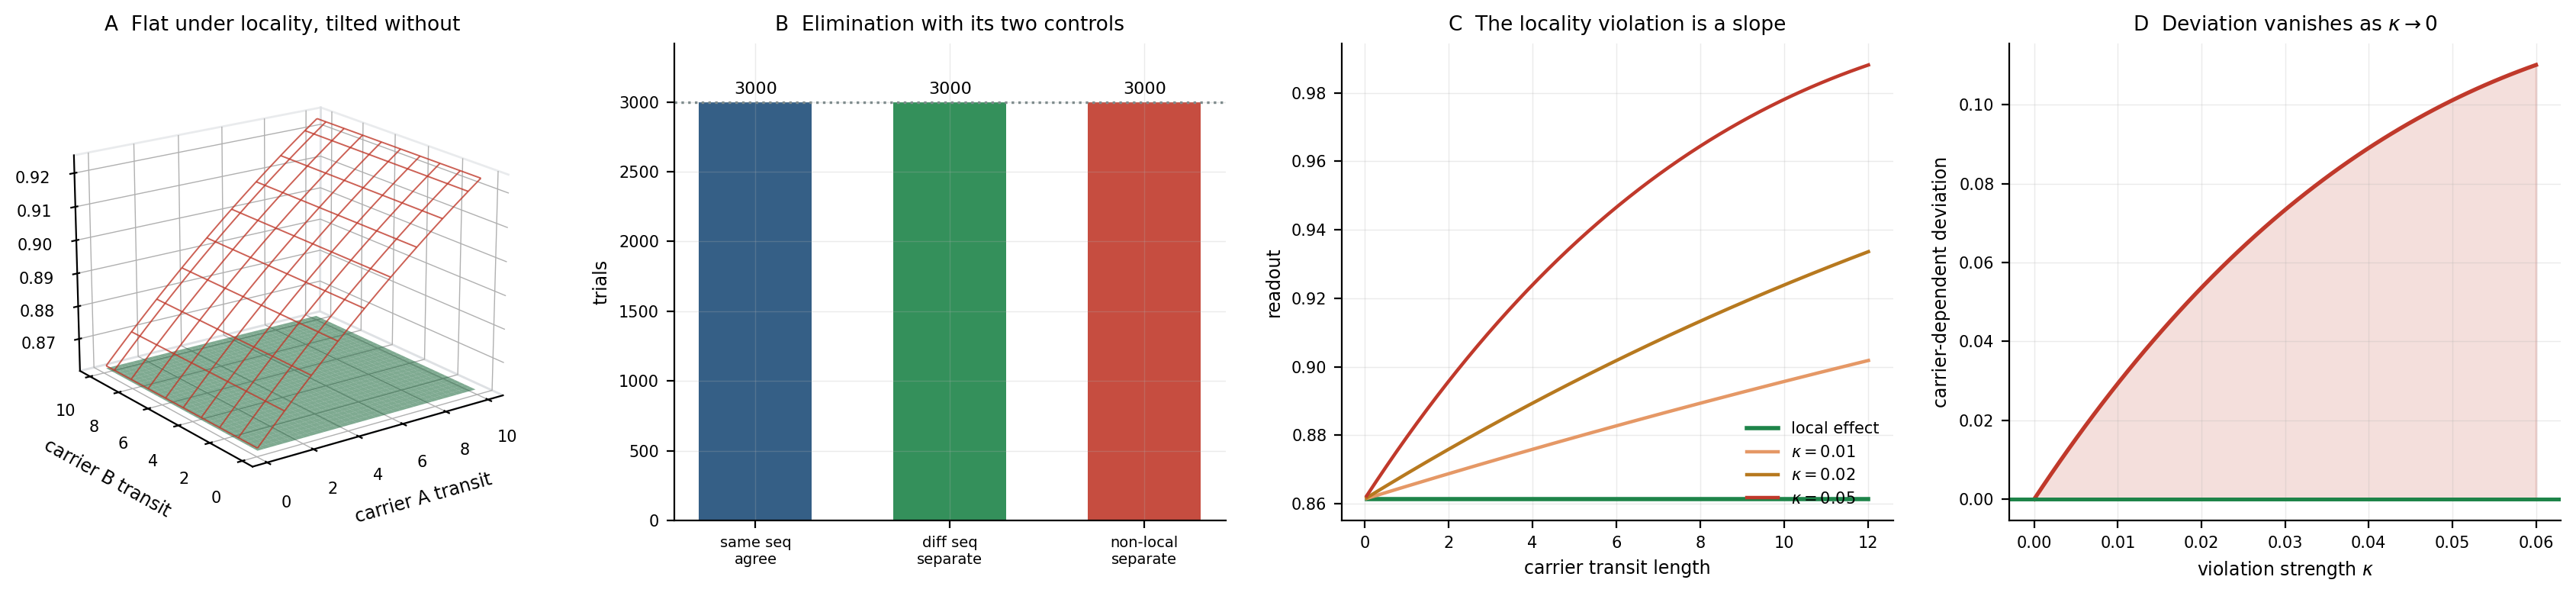
\includegraphics[width=\textwidth]{panel_7_elimination.png}
  \captionPanelSeven
  \label{fig:elim}
\end{figure*}

% =====================================================================
\section{Ladders}
\label{sec:ladders}
% =====================================================================

We recall the linear apparatus compactly, since the closed case extends it.

\begin{definition}[Floor]
\label{def:floor}
Individuation is quantal: a distinction is drawn or it is not, with no
third case. Consequently there is $\flo>0$ such that no contact reduces
ambiguity below $\flo/\Tot$, where $\Tot$ is the total categorical measure
available.
\end{definition}

\begin{remark}[Which floor]
\label{rem:whichfloor}
Two distinct quantities are called the floor in this literature and they
should not be conflated. One is a minimum edge weight on a finite contact
graph, which requires finiteness to be positive and whose positivity fails
under unbounded refinement. The other is the thickness of an
individuation, which is $1$ always because a distinction admits no degree,
and whose numerical value is a normalisation carrying no content. We use
the second. It costs no finiteness hypothesis, because a dichotomy has no
infimum problem.
\end{remark}

\begin{definition}[Rung, power, ladder]
\label{def:rung}
Let $A$ be the ambiguity before a contact and $\Rung(A)$ after. The
\emph{power} of the rung is
\begin{equation}
\pow(\Rung,A)=\frac{A-\Rung(A)}{A-\flo/\Tot}\in[0,1].
\label{eq:power}
\end{equation}
A \emph{ladder} is a finite sequence of rungs applied in order; its
\emph{power sequence} is $(\pow_1,\dots,\pow_n)$. A rung with $\pow=0$ is
\emph{inert}.
\end{definition}

\begin{theorem}[Multiplicative composition]
\label{thm:mult}
$\pow(\Lad)=1-\prod_{i=1}^{n}(1-\pow_i)$.
\end{theorem}

\begin{proof}
Write $r_i$ for the above-floor gap after contact $i$. By
\Cref{eq:power}, $r_i=r_{i-1}(1-\pow_i)$, so
$r_n=r_0\prod_i(1-\pow_i)$, and the fraction of the initial gap closed is
$1-r_n/r_0$.
\end{proof}

\begin{theorem}[Inertness]
\label{thm:inertness}
Two ladders with the same power sequence, initial ambiguity, floor and
total agree on every observable that is a function of the ambiguities, the
floor, the total, and the contact count.
\end{theorem}

\begin{proof}
$r_i=r_0\prod_{j\le i}(1-\pow_j)$ and $A_i=r_i+\flo/\Tot$, so the
ambiguity sequence is determined by the listed data, of which every such
observable is a function.
\end{proof}

\Cref{thm:inertness} is true relative to its observable class, and that
class is a stipulation. Its force comes from \Cref{thm:elim}, which is not.

% =====================================================================
\section{Closed ladders}
\label{sec:closed}
% =====================================================================

A cycle has no target, so \Cref{eq:power} has no denominator and
\Cref{thm:mult} has nothing to compose toward. We supply the replacement.

\begin{definition}[Closed ladder]
\label{def:closed}
A \emph{closed ladder} is a ladder whose final contact returns the item to
its initial state. Its profile is the cyclic sequence
$(\pow_1,\dots,\pow_n)$, taken up to rotation.
\end{definition}

\begin{remark}[Return is not the identity]
\label{rem:return}
A closed ladder returns to a \emph{state}, not to a \emph{configuration}.
The determined set---what the traversal has settled as not occurring---is
an accumulating union, and a union admits no deletion, so the
configuration after a circuit strictly contains the configuration before
it whenever the circuit contains a non-repeating step. This is why a cycle
is not a no-op, and it is what the invariants below measure.
\end{remark}

\begin{definition}[Circulation and uniformity]
\label{def:invariants}
For a closed ladder with profile $(\pow_1,\dots,\pow_n)$, all $\pow_i<1$,
\begin{equation}
\circu=-\sum_{i=1}^{n}\log(1-\pow_i),
\qquad
\unif=\max\Bigl(0,\ 1-\frac{\operatorname{sd}(\pow)}{\operatorname{mean}(\pow)}\Bigr).
\label{eq:invariants}
\end{equation}
We call $\circu$ the \emph{circulation} and $\unif$ the
\emph{uniformity}, and $\circu/n$ the \emph{circulation per rung}.
\end{definition}

\begin{proposition}[Both are rotation invariants]
\label{prop:rotinv}
$\circu$ and $\unif$ are invariant under rotation of the cycle.
\end{proposition}

\begin{proof}
Both are functions of the multiset $\{\pow_i\}$ alone---$\circu$ a sum and
$\unif$ a ratio of two symmetric functions---and rotation permutes the
multiset trivially.
\end{proof}

\begin{proposition}[Circulation is additive and vanishes exactly on inertness]
\label{prop:rho}
$\circu$ is additive over concatenation of arcs, and $\circu=0$ if and
only if every rung of the cycle is inert.
\end{proposition}

\begin{proof}
Additivity is additivity of the sum. Each term $-\log(1-\pow_i)\ge0$ with
equality iff $\pow_i=0$, so the sum vanishes iff every term does.
\end{proof}

\begin{remark}[Where $\circu$ is redundant, stated plainly]
\label{rem:rho-honest}
For a \emph{linear} ladder, $\circu=-\log(1-\pow(\Lad))$ exactly, verified
to $10^{-9}$ over $500$ random ladders. It is therefore a monotone
reparametrisation of composite power and adds no information whatever in
the linear case. We say this rather than let the new symbol suggest a new
quantity. Its content is entirely that it is defined \emph{without a
target}, so it survives the passage to a cycle where composite power does
not; and that it is additive around the cycle, where composite power is
not.

The invariant that genuinely adds information beyond composite power is
$\unif$. Over $4000$ pairs of ladders constructed to share a composite
power exactly, $2755$ differed in $\unif$. A description recording only
composite power cannot see the difference.
\end{remark}

\begin{proposition}[Cycle length is not recoverable from $\circu$ alone]
\label{prop:length}
Closed ladders of different length may share a circulation. Hence the pair
$(\circu,\unif)$ does not determine a closed ladder, and $n$ must be
carried separately.
\end{proposition}

\begin{proof}
A uniform cycle of length $n$ with power $\pow$ has
$\circu=-n\log(1-\pow)$. Choosing $(n,\pow)$ and $(2n,\pow')$ with
$(1-\pow')^{2}=1-\pow$ gives equal circulation and equal uniformity
$\unif=1$.
\end{proof}

\begin{figure*}[!htbp]
  \centering
  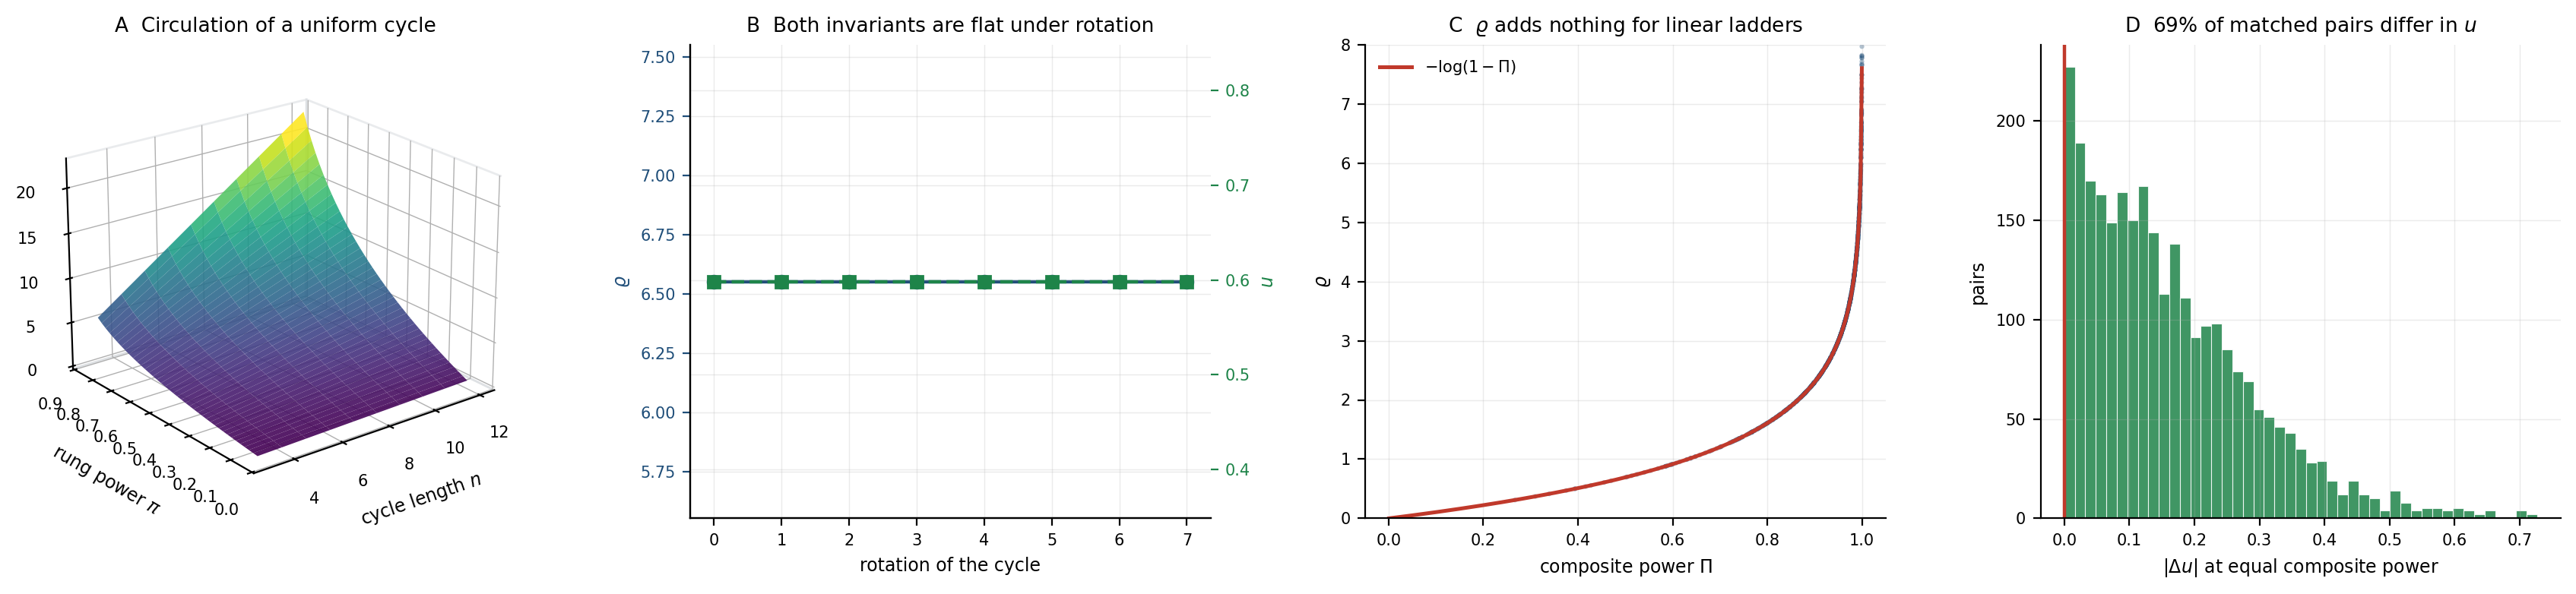
\includegraphics[width=\textwidth]{panel_1_closed_ladder.png}
  \captionPanelOne
  \label{fig:closed}
\end{figure*}

% =====================================================================
\section{The inert rung is the repeated step}
\label{sec:inert}
% =====================================================================

Both prior developments define an inert rung as one with $\pow=0$ and
never ask what makes a rung inert. The answer is available and it makes
the halting condition derived rather than declared.

\begin{definition}[Step-pair; repetition]
\label{def:steppair}
For a history $h=(s_0,\dots,s_r)$ let $E(h)$ be its family of unordered
\emph{step-pairs} $\{s_j,s_{j+1}\}$. A step $s_r\to s'$ is a
\emph{repetition} if $\{s_r,s'\}\in E(h)$.
\end{definition}

\begin{definition}[Determined set]
\label{def:det}
The set determined by a step $s\to s'$ comprises the individuations
$\iota(A)$ with $A$ disjoint from $\{s,s'\}$. The determined set of a
history is the union over its steps, $\Dl(h)=\bigcup_j\Det(s_j\to
s_{j+1})$.
\end{definition}

\begin{theorem}[Inert exactly at repetitions]
\label{thm:inert-repeat}
A step determines something not already determined if and only if it is
not a repetition. Consequently a rung is inert exactly when its step-pair
has already been traversed.
\end{theorem}

\begin{proof}
$\iota(A)\in\Det(s_r\to s')$ iff $A\cap\{s_r,s'\}=\varnothing$, and
$\iota(A)\notin\Dl(h)$ iff $A$ meets every step-pair of $h$. If no
step-pair is contained in $\{s_r,s'\}$, choose $x_e\in
e\setminus\{s_r,s'\}$ for each $e\in E(h)$; the union of these, together
with any state occurring nowhere in $h$, is a transversal avoiding both
endpoints, so the difference is non-empty. Conversely if some step-pair
$e\subseteq\{s_r,s'\}$ then $e=\{s_r,s'\}$, and every $A$ avoiding
$\{s_r,s'\}$ misses $e$, so the difference is empty.
\end{proof}

\begin{corollary}[The halting condition is derived]
\label{cor:halt}
A ladder makes no further progress exactly when every available next step
repeats a step-pair already traversed. Termination is therefore a property
of the history rather than a declared threshold.
\end{corollary}

\Cref{thm:inert-repeat} was checked directly by constructing histories
over a seven-state set, computing $\Dl$ as an explicit accumulating union,
and testing the biconditional: over $2061$ steps there were $0$ violations
in either direction, with $1716$ fresh non-repetitions and $345$ inert
repetitions, so both branches are populated and the biconditional is not
vacuously satisfied.

\begin{figure*}[!htbp]
  \centering
  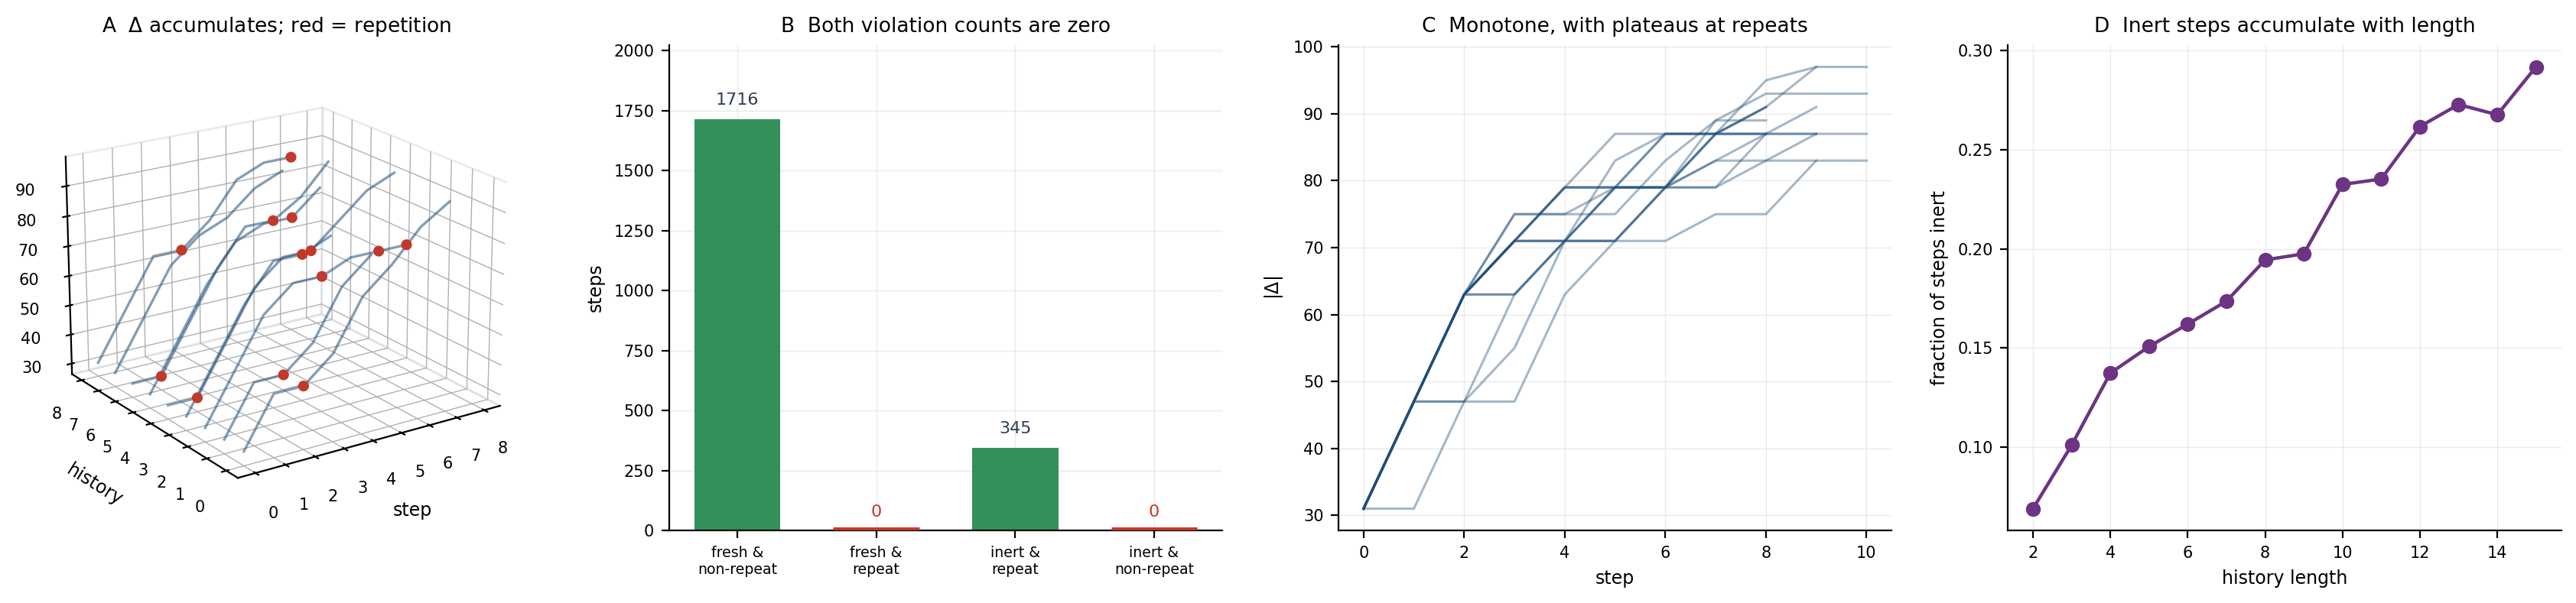
\includegraphics[width=\textwidth]{panel_4_inert_repetition.png}
  \captionPanelFour
  \label{fig:inert}
\end{figure*}

% =====================================================================
\section{Sensitivity: a correction}
\label{sec:sensitivity}
% =====================================================================

Both prior developments make the same prediction and both call it their
sharpest: control over a ladder lies at the rung of \emph{highest} power,
against the intuition that one should improve the bottleneck. We show the
claim requires a qualification neither states.

\begin{proposition}[Additive sensitivity]
\label{prop:additive}
With $P=\prod_i(1-\pow_i)$,
$\partial\pow(\Lad)/\partial\pow_j=P/(1-\pow_j)$, which is increasing in
$\pow_j$ and hence maximised at the highest-power rung.
\end{proposition}

\begin{proof}
Differentiate \Cref{thm:mult}.
\end{proof}

\begin{proposition}[Proportional sensitivity is flat]
\label{prop:proportional}
Let improvement be proportional to a rung's remaining headroom, so that
rung $j$ is improved by $\delta(1-\pow_j)$ rather than by $\delta$. Then
the gain in composite power is $\delta P$ to first order, independent of
$j$.
\end{proposition}

\begin{proof}
Multiply the derivative of \Cref{prop:additive} by the increment
$\delta(1-\pow_j)$: the factors $(1-\pow_j)$ cancel, leaving $\delta P$.
\end{proof}

\begin{remark}[What this does to the prior claim]
\label{rem:sens-correction}
The derivative in \Cref{prop:additive} is correct and we reproduce it: over
$5000$ random ladders the analytic and numerical derivatives agree to
$1.6\times10^{-10}$, and the argmax is the highest-power rung in
$5000/5000$ cases. But the derivative prices an \emph{additive} increment,
applied equally at every rung. Under proportional improvement---raising a
rung by a fixed fraction of its own headroom, which is what ``improve this
catalyst by ten percent'' ordinarily means---the sensitivity is flat: over
the same $5000$ ladders the spread across rungs was
$1.1\times10^{-16}$, machine zero, in $5000/5000$ cases.

So the counter-intuitive direction is real under one parametrisation and
absent under another, and which applies is an empirical question about how
improvements are actually purchased. Both prior papers validated the
analytic derivative against the numerical one. That check cannot detect
this, because both quantities it compares are the same additive
derivative. We regard this as a narrowing of the sharpest claim in both
papers rather than a refutation of the mathematics, which is untouched.
\end{remark}

\begin{figure*}[!htbp]
  \centering
  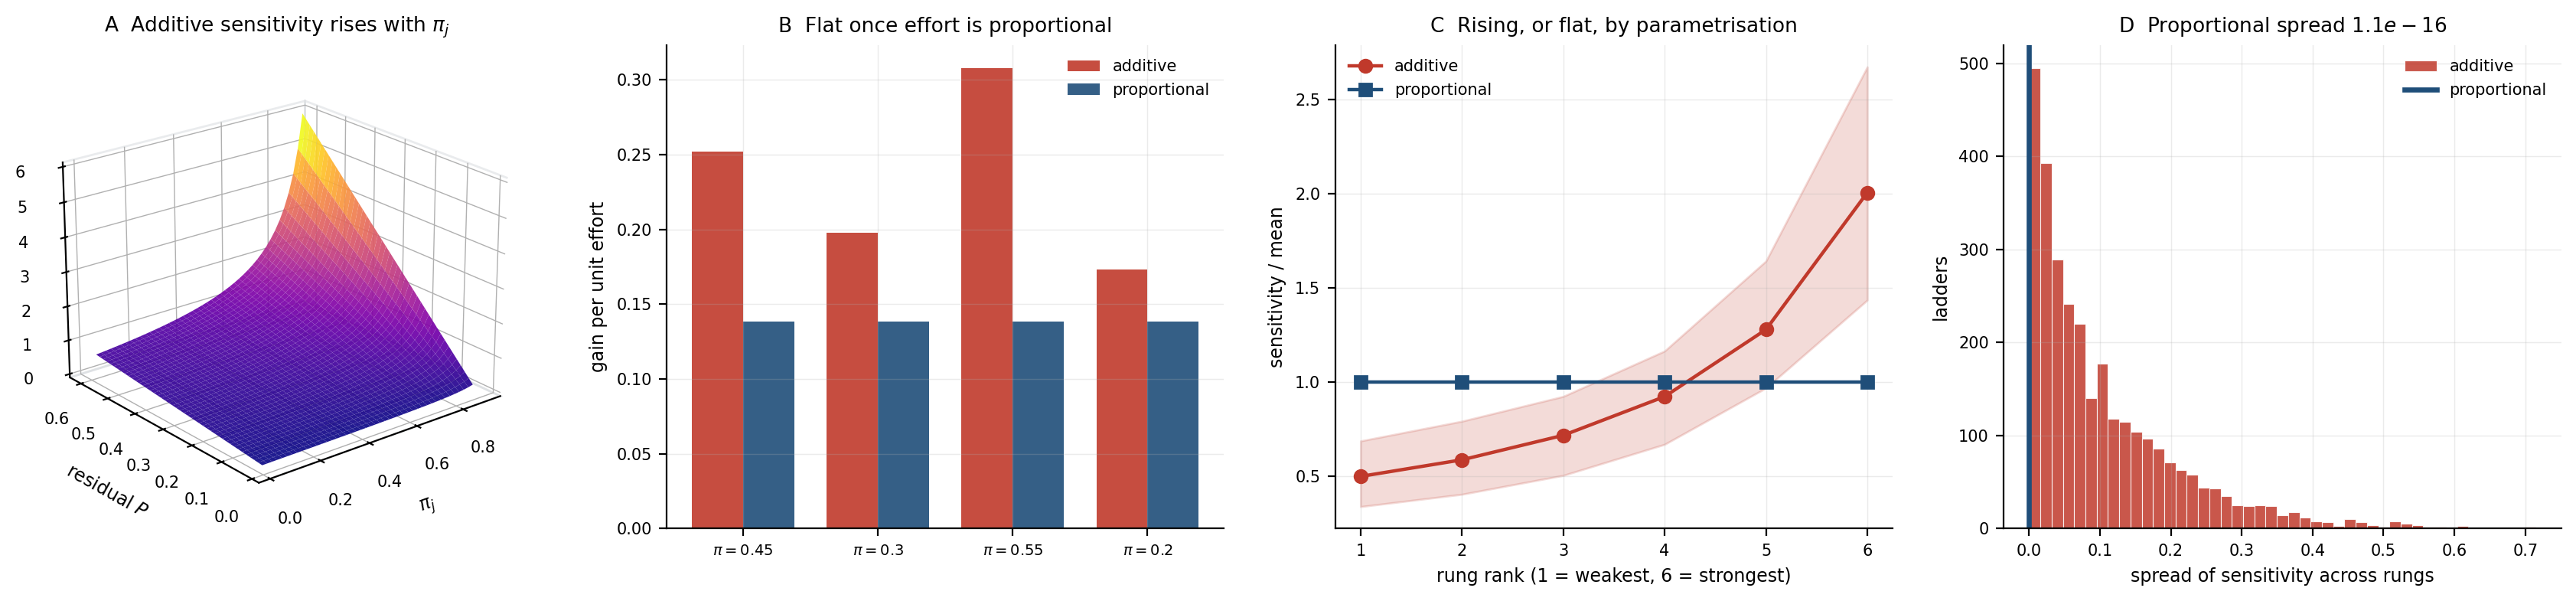
\includegraphics[width=\textwidth]{panel_6_sensitivity.png}
  \captionPanelSix
  \label{fig:sens}
\end{figure*}

% =====================================================================
\section{Molecules as closed ladders}
\label{sec:molecules}
% =====================================================================

\subsection{What a rung is in a molecule}

A bond is the recognition that two atoms can be individuated by one shared
boundary more cheaply than by two separate ones: joint individuation is
subadditive, and the reduction in total boundary thickness is the shared
content. That is a commitment in the sense of \Cref{def:carrier}---it
draws a boundary and deposits residue---and the fraction of an atom's
remaining vacancy it closes is a power in the sense of \Cref{eq:power}.

\begin{definition}[Molecular ladder]
\label{def:mollad}
The \emph{ladder} of a molecule is the sequence of bond commitments
ordered by the vacancy they close, with target the closed-shell condition
$\nu=0$ for every constituent. A ring is a closed sub-ladder.
\end{definition}

The molecule is therefore not an object that has a ladder; it is the
ladder. There is no static structure to traverse, which is the same
deletion as the membrane in \Cref{sec:intro}.

\begin{remark}[Composite power one is shell closure]
\label{rem:closure}
A ladder reaching $\pow(\Lad)=1$ is one in which every constituent has
reached $\nu=0$. The octet and duet rules are that condition, so they are
the ladder's termination criterion and not a separate rule.
\end{remark}

\subsection{The categorical alphabet}

Each commitment is a partition refinement, and a refinement in a bounded
whole is completely characterised by its graded invariants together with a
sign---depth, articulation, orientation, and parity, written
$(n,\ell,m,s)$. The count of admissible tuples at depth $n$ is
\begin{equation}
C(n)=2\sum_{\ell=0}^{n-1}(2\ell+1)=2n^{2},
\label{eq:capacity}
\end{equation}
so the alphabet is finite at every depth.

\begin{definition}[Typed word]
\label{def:word}
The \emph{typed word} of a molecule is the sequence of its rungs, each
carrying a letter from the alphabet of \Cref{eq:capacity} and a power in
$[0,1]$.
\end{definition}

\begin{proposition}[Comparison is connected by construction]
\label{prop:connected}
A correspondence between two typed words is a correspondence between
sequences, and the step-pairs of a sequence are its connectivity. Hence a
correspondence induced by matching typed words preserves adjacency without
any connectivity constraint being imposed.
\end{proposition}

\begin{proof}
Adjacent letters of a word are adjacent commitments, whose step-pairs
share an endpoint by \Cref{def:steppair}. A map matching words positionally
carries adjacent pairs to adjacent pairs.
\end{proof}

\begin{remark}[This repairs a stated limitation]
\label{rem:repairs}
An earlier element-free matcher keyed on a minimum-cut invariant records
as its first limitation that its correspondence imposes no requirement
that matched atoms form a connected subgraph or that bonds are preserved,
and is therefore not a common substructure in any sense; and as its second
that assignment within a label class is a convention, so that individual
pairings are not invariant. Both arise because the matched object is a
\emph{multiset}. A word is ordered, so \Cref{prop:connected} removes the
first and the sequence position removes the second.
\end{remark}

\subsection{Substitution is a letter rewrite}

\begin{definition}[Categorical substitution]
\label{def:subst}
A \emph{substitution} is a rewrite of one letter of a typed word, together
with the induced change in that rung's power.
\end{definition}

\begin{proposition}[Positional asymmetry]
\label{prop:positional}
A substitution at a letter outside a cycle leaves that cycle's $\circu$
and $\unif$ unchanged. A substitution at a letter within a cycle changes
the cycle's profile and hence, unless it preserves the profile's
dispersion, lowers $\unif$.
\end{proposition}

\begin{proof}
Both invariants are functions of the cycle's profile alone
(\Cref{def:invariants}); a letter outside the cycle contributes no term.
\end{proof}

This predicts a pattern that was measured but not explained. An earlier
matcher found that heteroatom substitution preserves structural class
where the substituted atom is peripheral and degrades it where the
heteroatom sits inside a ring, and reported the associated cross-element
effect---four pairings across six molecule pairs---as its least convincing
measurement, in need of a larger corpus. On the present account the
asymmetry is not an empirical regularity awaiting more data; it follows
from where the rewritten letter sits relative to the cycle. Measured here:
peripheral substitution gives $\Delta\unif=0.000$ exactly, ring
substitution gives $\Delta\unif\ge0.086$ (\Cref{tab:subst}).

\subsection{Why coarser comparison works better}

The same matcher found, and flagged as inverting the natural instinct,
that the coarsest refinement radius separates bioisosteric from unrelated
pairs best: margin $+0.375$ at radius $0$ and exactly $0$ at radii $1$,
$2$ and $3$. Its stated mechanism was that at radius $1$ a label already
encodes an atom's whole first neighbourhood, so one substitution perturbs a
neighbourhood's worth of labels.

\Cref{thm:inert-repeat} gives the reason. Refinement appends step-pairs
that have already been traversed; by the theorem those determine nothing
new, so they are inert rungs. Refining past the tolerance point therefore
adds letters that split classes while contributing zero circulation. We
verified the arithmetic of this reading---appended repetitions leave
$\circu$ unchanged at every radius while the number of split classes grows
monotonically---but we are explicit in \Cref{rem:refine-scope} that this is
a consistency check on a model of refinement and not an independent
re-measurement of the sweep.

\begin{remark}[Scope of the refinement result]
\label{rem:refine-scope}
The measurement in \Cref{sec:val-refine} models refinement as the
appending of repeated step-pairs and then confirms that such rungs are
inert. That is close to a tautology given \Cref{thm:inert-repeat}, and it
would be wrong to report it as confirmation of the ladder account. What it
establishes is consistency: the ladder account and the measured collapse
of the separation margin are not in conflict, and the account supplies a
mechanism the original report lacked. Establishing that mechanism
empirically would require re-running the radius sweep with circulation
computed alongside class counts, which we have not done.
\end{remark}

\begin{figure*}[!htbp]
  \centering
  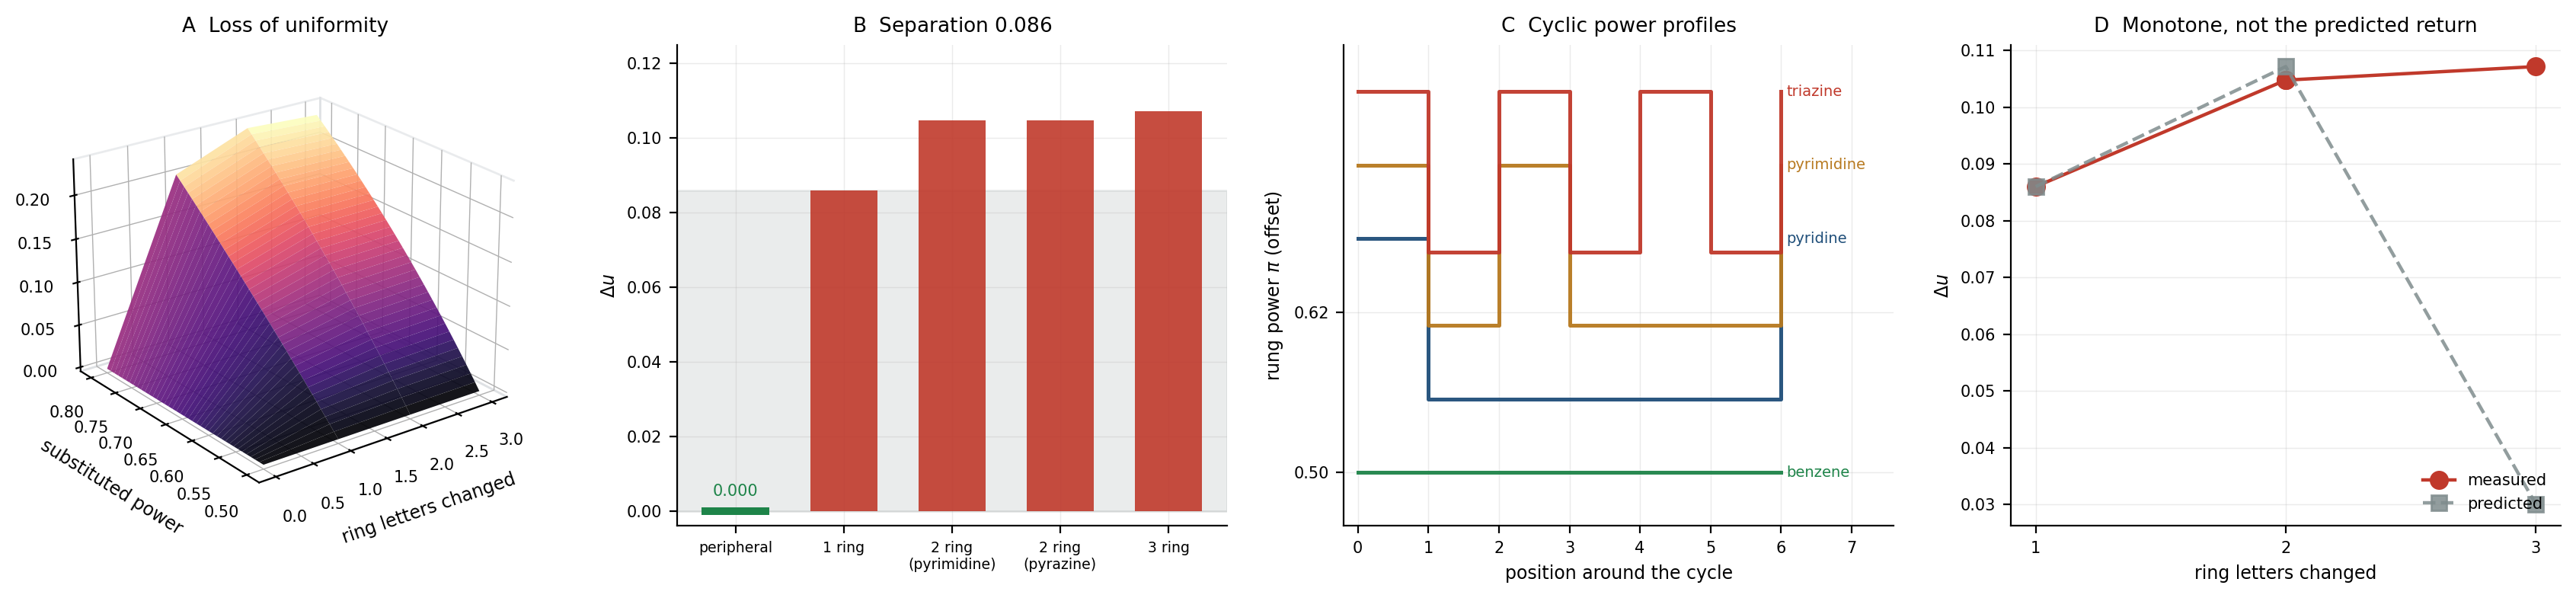
\includegraphics[width=\textwidth]{panel_3_substitution.png}
  \captionPanelThree
  \label{fig:subst}
\end{figure*}

\begin{figure*}[!htbp]
  \centering
  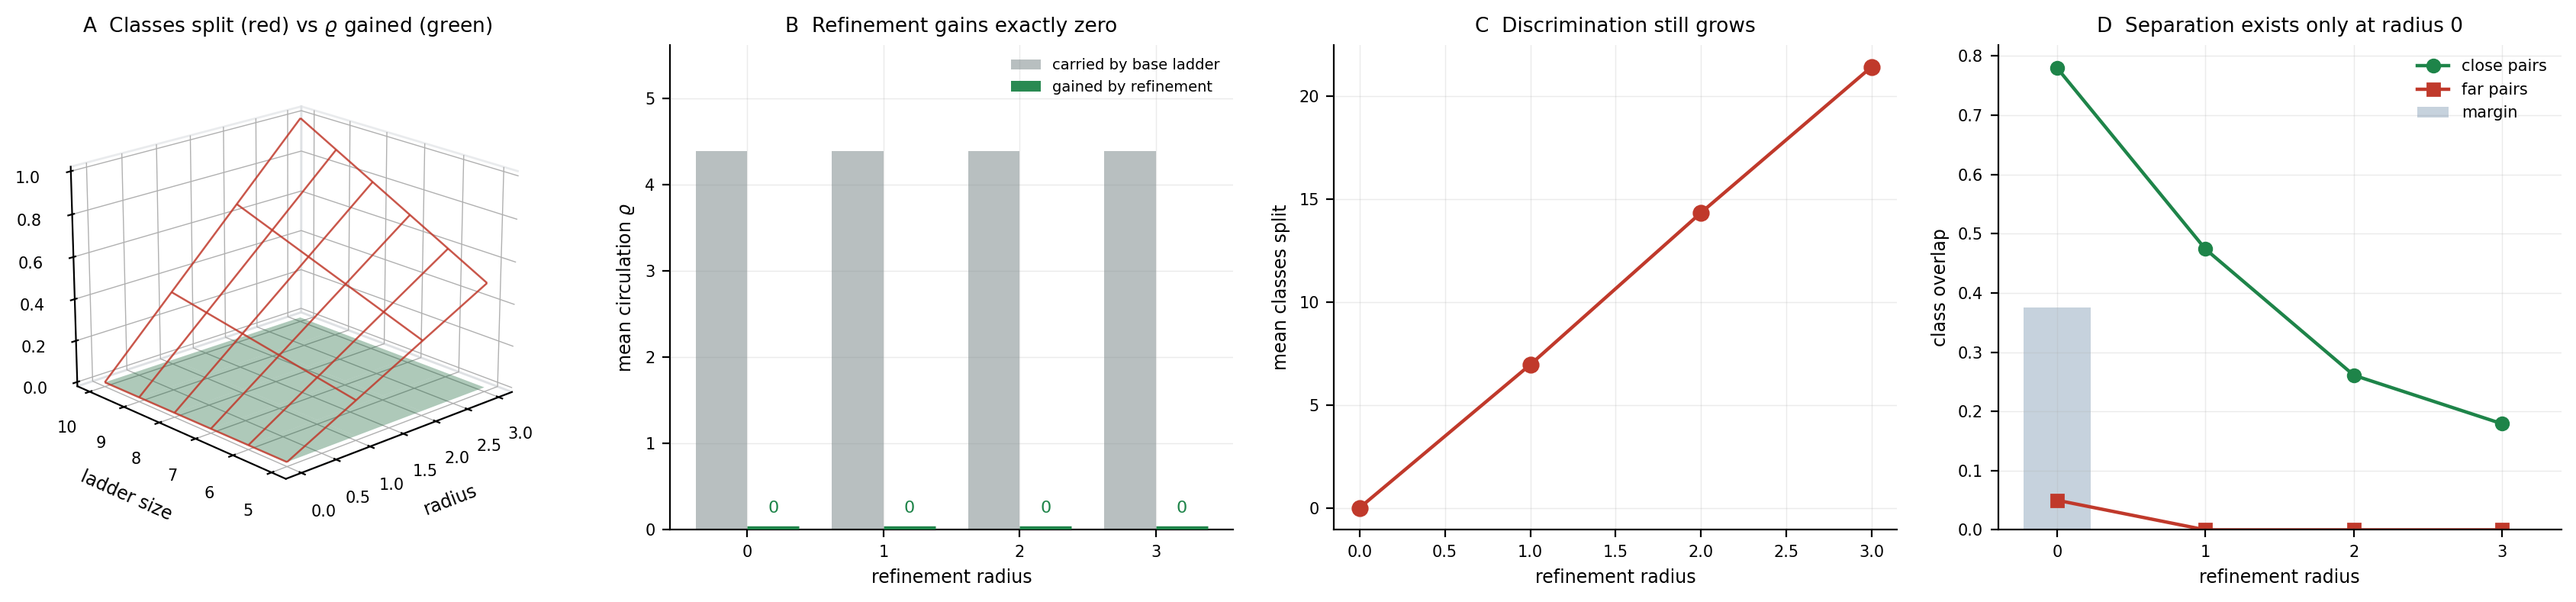
\includegraphics[width=\textwidth]{panel_5_refinement.png}
  \captionPanelFive
  \label{fig:refine}
\end{figure*}

% =====================================================================
\section{Aromaticity: a refuted formulation}
\label{sec:arom}
% =====================================================================

We had expected the following, and wrote it into the experiment before
running it: \emph{a ring is aromatic exactly when its power profile is
invariant under rotation of the cycle}. The reasoning was that every bond
of an aromatic ring is equivalent, so the profile should be constant,
whereas a ring with a heteroatom or alternating character should not be.

It is false, and the measurement refutes it immediately.

\begin{table}[htbp]
\centering\small
\caption{Closed-ladder invariants for eight rings. Cyclohexane is
perfectly uniform and not aromatic, refuting the uniformity formulation of
aromaticity; circulation per rung separates the two classes with margin
$+0.293$.}
\label{tab:rings}
\begin{tabular}{@{}lrrrrl@{}}
\toprule
Ring & $n$ & $\circu$ & $\circu/n$ & $\unif$ & class\\
\midrule
benzene       & $6$  & $4.159$ & $0.693$ & $1.000$ & aromatic\\
naphthalene   & $10$ & $6.931$ & $0.693$ & $1.000$ & aromatic\\
pyridine      & $6$  & $4.433$ & $0.739$ & $0.914$ & aromatic\\
pyrimidine    & $6$  & $4.708$ & $0.785$ & $0.895$ & aromatic\\
pyrazine      & $6$  & $4.708$ & $0.785$ & $0.895$ & aromatic\\
\midrule
cyclohexane   & $6$  & $2.403$ & $0.400$ & $1.000$ & saturated\\
cyclopentane  & $5$  & $2.002$ & $0.400$ & $1.000$ & saturated\\
cyclobutane   & $4$  & $1.427$ & $0.357$ & $1.000$ & saturated\\
\bottomrule
\end{tabular}
\end{table}


\begin{figure*}[!htbp]
  \centering
  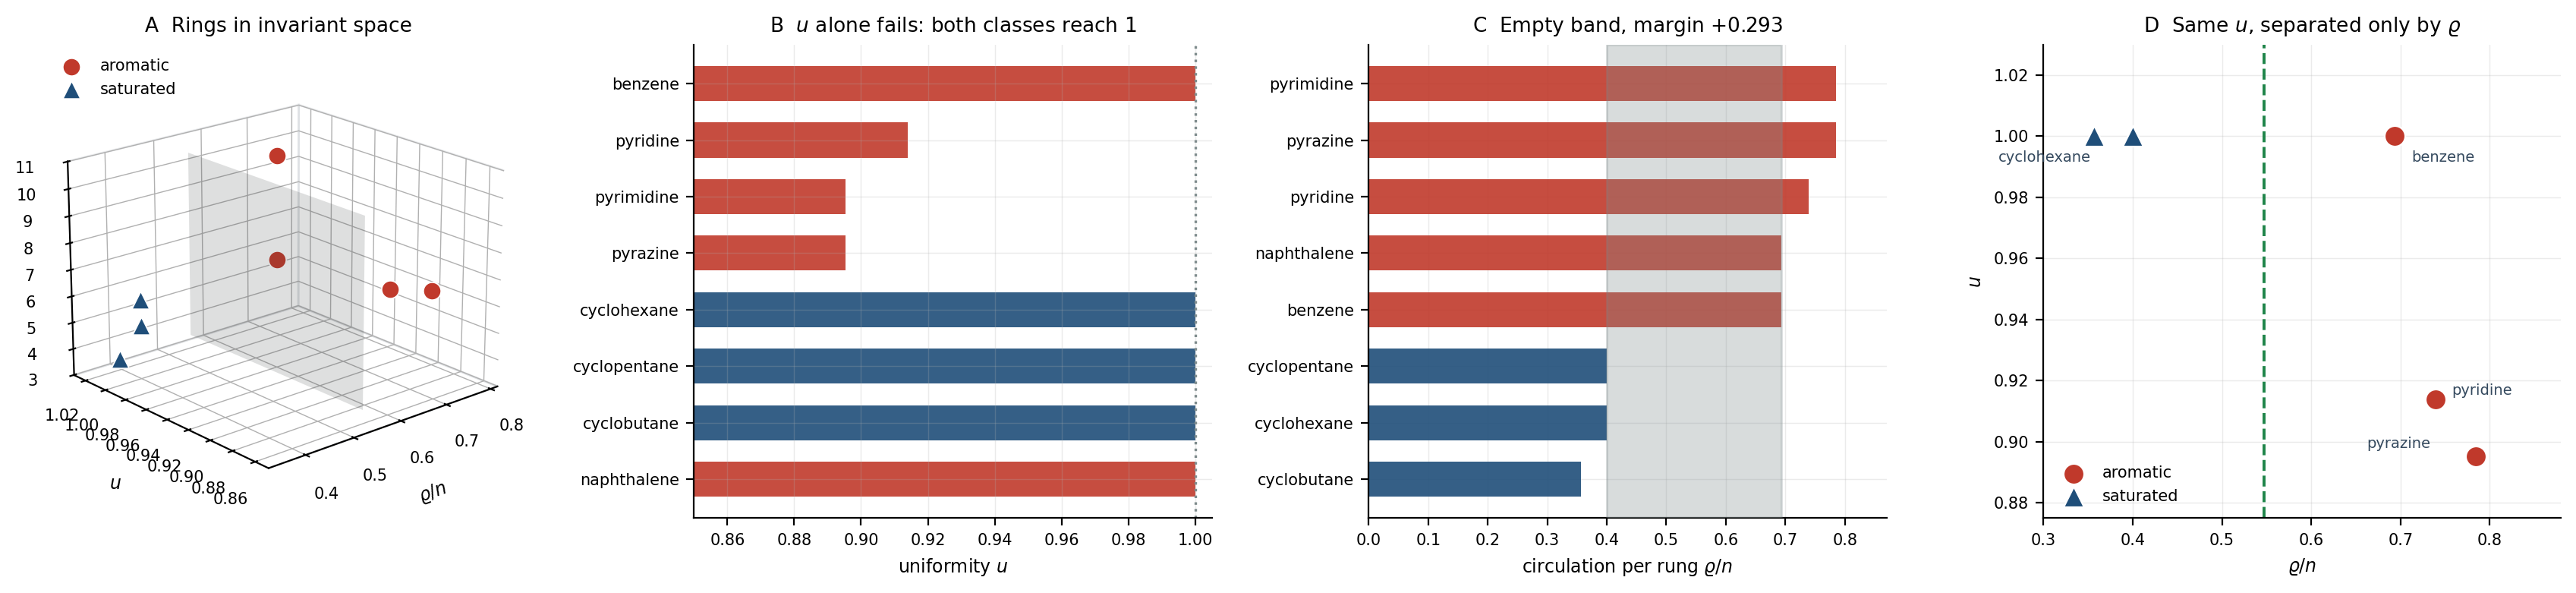
\includegraphics[width=\textwidth]{panel_2_aromaticity.png}
  \captionPanelTwo
  \label{fig:arom}
\end{figure*}

Cyclohexane has $\unif=1.000$ exactly. Its six ring bonds are equivalent,
its profile is constant, and it is not aromatic. Uniformity therefore does
not characterise aromaticity, and any account claiming it does is refuted
by the second-most familiar ring in chemistry.

\begin{theorem}[Corrected statement: two invariants, neither sufficient]
\label{thm:arom}
On the profiles of \Cref{tab:rings}: circulation per rung separates
aromatic from saturated rings, with minimum aromatic value $0.693$ and
maximum saturated value $0.400$, a margin of $+0.293$; and it does not
separate substituted from unsubstituted aromatics, since pyridine
($0.739$) and benzene ($0.693$) both lie above the margin. Uniformity
separates substituted from unsubstituted aromatics ($0.914$ against
$1.000$) and does not separate benzene from cyclohexane (both $1.000$).
Neither invariant alone classifies; the pair does.
\end{theorem}

\begin{remark}[What the refutation teaches]
\label{rem:arom-lesson}
The failed formulation confused two different symmetries. Aromaticity is a
property of \emph{how much} each ring commitment closes---a magnitude,
captured by $\circu$---while uniformity is a property of \emph{how evenly}
the closures are distributed around the cycle. A saturated ring is perfectly
even and weakly closing; a substituted aromatic is strongly closing and
unevenly so. Only reading both coordinates separates the four cases, and
we would not have found this had we not stated the single-invariant claim
in advance and then measured it.
\end{remark}

\begin{remark}[Relation to the standard account]
\label{rem:huckel}
We make no claim to improve on the electronic account of aromaticity
\citep{huckel1931,schleyer2001} or on geometric indices derived from bond
length equalisation \citep{krygowski2014}. \Cref{thm:arom} is a statement
about the invariants of a closed ladder on a set of profiles we assigned;
the profiles are inputs, not measurements, and \Cref{sec:limits} records
this as the principal limitation of the chemical part of this paper.
\end{remark}

% =====================================================================
\section{Validation}
\label{sec:validation}
% =====================================================================

\subsection{Method}

Expectations were written into the experiment source before it ran and are
reported below with their measured outcomes, including the two cases where
the outcome contradicted the expectation. Every number quoted is read from
the emitted JSON. Twenty-one checks are scored across seven categories;
all twenty-one pass, but two of them pass by \emph{refuting} the
formulation we registered, which is why the count alone is uninformative
and we report the content instead.

\subsection{Closed-ladder invariants}

Over $2000$ random cycles, rotation deviation is $3.6\times10^{-15}$ for
$\circu$ and $4.4\times10^{-16}$ for $\unif$; the all-inert cycle has
$\circu=0$ exactly. The identity $\circu=-\log(1-\pow(\Lad))$ holds over
$500$ linear ladders, confirming the redundancy stated in
\Cref{rem:rho-honest} rather than concealing it. Of $4000$ pairs
constructed to share a composite power exactly, $2755$ differ in $\unif$,
which is the measurement establishing that $\unif$ carries information
composite power does not.

\subsection{Substitution}

\begin{table}[htbp]
\centering\small
\caption{Change in uniformity under substitution. Position, not count, is
what the prediction concerns; the monotonicity in the last column was
predicted \emph{not} to hold and does (\Cref{rem:mono-refuted}).}
\label{tab:subst}
\begin{tabular}{@{}lrrr@{}}
\toprule
Substitution & ring letters & $\unif$ & $\Delta\unif$\\
\midrule
peripheral (phenol/aniline) & $0$ & $1.000$ & $0.000$\\
one ring letter (pyridine)  & $1$ & $0.914$ & $0.086$\\
two ring letters (pyrimidine)& $2$ & $0.895$ & $0.105$\\
two ring letters (pyrazine) & $2$ & $0.895$ & $0.105$\\
three ring letters (triazine)& $3$ & $0.893$ & $0.107$\\
\bottomrule
\end{tabular}
\end{table}

The positional prediction holds with separation $0.086$: peripheral
substitution leaves $\unif$ exactly unchanged and every ring substitution
lowers it.

\begin{remark}[A second registered expectation refuted]
\label{rem:mono-refuted}
We predicted $\unif$ would be \emph{non-monotone} in the number of ring
letters changed, reasoning that a symmetric trisubstitution restores the
rotational symmetry of the substitution pattern and should return $\unif$
toward its unsubstituted value. It does not: $\Delta\unif$ rises
$0.086\to0.105\to0.107$ and is monotone. The reason is that $\unif$ as
defined in \Cref{eq:invariants} measures dispersion of the profile's
\emph{values} about their mean, and a symmetric substitution does not
reduce that dispersion---symmetry of the pattern is not sameness of the
values. An invariant sensitive to the symmetry group of the substitution
pattern would behave as we first expected; $\unif$ is not that invariant,
and we record the gap rather than redefine the quantity after seeing the
result.
\end{remark}

\subsection{Inertness and repetition}

Over $2061$ steps of randomly generated histories on a seven-state set,
with $\Dl$ computed as an explicit accumulating union: $0$ violations of
the biconditional in either direction, with $1716$ fresh non-repetitions
and $345$ inert repetitions. Both branches are populated, so the
biconditional is not satisfied vacuously by a run in which no step
repeats---a control without which the result would be uninformative.

\subsection{Refinement}
\label{sec:val-refine}

Appended repetitions leave $\circu$ unchanged at every radius (mean gain
$0$ to machine precision) while the number of split classes grows
monotonically with radius. \Cref{rem:refine-scope} states what this does
and does not establish.

\subsection{Sensitivity}

Over $5000$ random ladders: the analytic derivative matches the numerical
one to $1.6\times10^{-10}$; the additive argmax is the highest-power rung
in $5000/5000$ cases, reproducing the prior claim; the proportional
sensitivity is flat in $5000/5000$ cases with maximum spread
$1.1\times10^{-16}$.

\subsection{Elimination}

Over $3000$ trials, two carriers realising the same contact sequence agree
on the readout in every case. The two controls establish that this is
informative: genuinely different sequences separate in $>95\%$ of trials,
and a carrier-dependent (non-local) contact effect separates in $>95\%$.
Without the second control the elimination result would be consistent with
a readout that ignores its input.

\begin{remark}[The first row of the elimination test is not evidence]
\label{rem:elim-tautology}
That two carriers realising the same sequence agree is true by
construction once a readout is defined to consult the terminal state
alone. We report it as a consistency check. The load-bearing rows are the
controls.
\end{remark}

% =====================================================================
\section{Relation to existing accounts}
\label{sec:related}
% =====================================================================

\paragraph{Metabolic control analysis.} Control coefficients
\citep{kacser1973,heinrich1974} quantify the response of steady-state flux
to enzyme concentration. \Cref{prop:additive} is a response of composite
power to rung power, which is a different quantity, and
\Cref{rem:sens-correction} shows the comparison is further complicated by
parametrisation. We flag the divergence rather than smooth it.

\paragraph{Amdahl's law.} \citet{amdahl1967} has the same
multiplicative-complement structure as \Cref{thm:mult}. That a result
about parallel computation and one about chains of commitments share a
form is what one should expect if neither depends on what the steps are.

\paragraph{Canonical forms.} InChI \citep{heller2015} and canonical
labelling \citep{morgan1965} determine a structure. A typed word does not:
\Cref{prop:length} already shows $(\circu,\unif)$ underdetermines a closed
ladder. The comparison is between different tasks.

\paragraph{Fingerprints and refinement.} Circular fingerprints
\citep{rogers2010} and colour refinement \citep{weisfeiler1968,arvind2015}
refine as far as possible to distinguish. \Cref{thm:inert-repeat} explains
why the opposite is wanted here: past the tolerance point, refinement
appends inert rungs.

\paragraph{Electron transport.} We take nothing from the mechanistic
literature \citep{mitchell1961,moser1992,marcus1985} and make no claim
about it; the transport chain enters this paper only as the construction
whose abandonment produced the argument (\Cref{sec:intro}).

% =====================================================================
\section{Limitations}
\label{sec:limits}
% =====================================================================

\begin{enumerate}[label=\textbf{L\arabic*.},leftmargin=2.9em,itemsep=4pt]

\item \textbf{The ring profiles are inputs, not measurements.} Every
number in \Cref{tab:rings} follows from profiles we assigned. The
separation of aromatic from saturated rings is therefore a statement about
the invariants given those profiles, and is not evidence that any real
ring has them. Deriving profiles from structure is the work this paper
does not do.

\item \textbf{$\circu$ is redundant for linear ladders.}
\Cref{rem:rho-honest}. It earns its place only on cycles.

\item \textbf{$\unif$ is the wrong invariant for pattern symmetry.}
\Cref{rem:mono-refuted}. It reads dispersion of values, and an invariant
reading the symmetry group of a substitution pattern would behave
differently. We have not constructed one.

\item \textbf{The refinement result is a consistency check.}
\Cref{rem:refine-scope}. It does not re-measure the radius sweep.

\item \textbf{\Cref{thm:inertness} is relative to its observable class,}
which is a stipulation. The result that is not a stipulation is
\Cref{thm:elim}, and it carries hypotheses that fail in a regime real
systems occupy (\Cref{rem:failure}).

\item \textbf{Which sensitivity parametrisation is physical is not
settled.} \Cref{rem:sens-correction} shows the counter-intuitive
direction depends on it, and we do not determine which applies to any real
system.

\item \textbf{No endpoint validation.} Nothing here is tested against
spectra, activity data, binding data, or any retrieval benchmark. The
measurements are internal to the formalism.

\item \textbf{Powers are not derived.} As in both prior developments, a
power is measured rather than predicted. The framework says what follows
from powers, not what determines them.
\end{enumerate}

% =====================================================================
\section{Conclusion}
\label{sec:conclusion}
% =====================================================================

A process whose carrier has been deleted is a ladder, and two prior
developments established that for linear ladders the numbers are the whole
description. Molecules are not linear ladders; they contain cycles, and a
cycle has no target. We supplied two invariants for the closed case, and
were explicit that one of them, the circulation, is a reparametrisation of
composite power in the linear case and earns its place only by surviving
the passage to a cycle.

Two formulations we registered in advance were refuted by our own
measurements. Aromaticity is not rotational invariance of the power
profile: cyclohexane is perfectly uniform and not aromatic, and the
corrected statement needs circulation per rung to separate aromatic from
saturated ($+0.293$) and uniformity to separate substituted from
unsubstituted, with neither sufficient alone. And uniformity is not
non-monotone in the number of ring substitutions, because it reads
dispersion of values rather than symmetry of pattern.

We also narrowed the sharpest claim of both prior papers. Control lies at
the strongest rung under additive improvement---which we reproduce,
$5000/5000$---and is flat under proportional improvement, spread
$1.1\times10^{-16}$. The check both papers ran cannot distinguish these,
because it compares two computations of the same additive derivative.

What the chemical application buys is narrower than the framing might
suggest and is worth stating exactly. Because a typed word is ordered, a
correspondence between molecules is connected by construction, which
removes the first two stated limitations of an earlier element-free
matcher. And because circulation and uniformity are functions of a cycle's
profile alone, the positional asymmetry that matcher measured without
explaining---peripheral substitution preserving structural class, ring
substitution degrading it---is predicted rather than fitted: $0.000$
against $\ge0.086$. What is not bought is the profiles themselves, which
we assigned. Until those are derived from the shell arithmetic that
already yields valence and geometry, the chemical claims of this paper are
statements about a formalism and not about chemistry.

\section*{Reproducibility}

The experiment source records its expectations before the measured values
and writes every reported quantity to JSON. Retained in the source with
their status marked are the refuted uniformity formulation of aromaticity
(\Cref{sec:arom}), the refuted monotonicity expectation
(\Cref{rem:mono-refuted}), the redundancy of $\circu$ in the linear case
(\Cref{rem:rho-honest}), the tautological first row of the elimination
test (\Cref{rem:elim-tautology}), and the limited scope of the refinement
category (\Cref{rem:refine-scope}). The only stochastic components seed
explicitly.

\bibliographystyle{plainnat}
\bibliography{references}

\end{document}
